%% Copyright (C) 2009 by Tobias Elze
%% Journal of Vision LaTeX template version 1.0
%% This document may be used freely for your own submissions.

\documentclass{jov}
\usepackage{graphicx} % needed for figures
\usepackage{subcaption}
\usepackage{hyperref}
\usepackage{amsmath}
\usepackage{bbm}
\usepackage{amssymb}
\usepackage{comment}

\DeclareMathOperator*{\argmin}{arg\,min}

\begin{document}

\title{Lightness constancy under fixed geometry}
\abstract{The light that reflects off an object surface and is captured by our eyes varies significantly with its context. But, the human visual system has the ability to stably perceive the object's color invariant of the context variations. The mechanism of this behaviorally significant invariance detection ability remains largely unknown. To understand the computational principles that lead to such invariant perception, we study the perception of object lightness under spectral variations in 3D scenes. Specifically, we study the effects of variations in reflectance and illumination spectra in a scene on the perceived lightness of an object. We have developed a software that generates naturalistic multispectral images of 3D scenes with precise control over the geometrical and spectral properties of the constituents that make a scene. We label these images with the lightness of a specific object in the scene. Next, we simulate the response of the retinal cones to these multispectral images using an accurate model of the early visual system.  Using supervised learning methods on these labeled cone response, we identify the computations that lead to accurate lightness estimation. We show that if only either target, or background, or illumination spectra are allowed to vary, the standard lightness can be estimated through simple transformations of the cone responses. When all the spectra vary simultaneously, while it is not easy to recover the lightness through simple transformations, a decoding scheme that compares the light from the target and the surround, and properly adds the response of the L,M and S cones can recover the lightness within about 15\% RMSE.}

\author{Singh}{Vijay}
 {Computational Neuroscience Initiative}
 {and Department of Physics, University of Pennsylvania, PA, USA}
 {}{vsin@sas.upenn.edu}

\keywords{color constancy, accuracy maximization analysis, supervised learning,
lightness}

\maketitle

\section{Introduction}
The perceived color of an object has important behavioral implications, since color helps us to identify objects and their properties \cite{Mollon89, Jacobs81}.
Perceived object color is not sensed directly, rather it is computed by the brain starting with the retinal image of light reflected from the object to the eye.
The challenge of object color perception is that this reflected light depends not just on the object's surface reflectance, but also on extrinsic factors such as the illumination, the object's pose,
and the position of the observer (Fig. \ref{fig:introSchematic}).
Thus, to produce a stable perceptual representation of an object's surface reflectance in the face of variation in these extrinsic factors, the brain must account for their influence on the reflected light.
The ability of a visual system to extract such a stable representation is called color constancy. Although human color constancy is by no means perfect, it is often very good \cite{FosterColorConstancy, BrainardColorConstancy}. 
In this paper, we consider the computational problem of color constancy, that is, how in principle could a visual system process the light reflected to the eyes to produce percepts well-correlated with object surface reflectance.

There is a considerable literature on computational color constancy. Seminal work considered a reduced scene model in which flat matte surfaces were illuminated by a single spatially diffuse illuminant and explored algorithms that could either recover a descriptor correlated with object surface reflectance (e.g. \citeNP{LandRetinex}) or explicit estimates of object surface reflectance and/or illuminant spectral power distribution (e.g., \citeNP{LandRetinex,Buchsbaum80,MaloneyWandell86}).
An important insight of this line of research was that, to account for variation in illumination, it was necessary to consider the light reflected from the entire scene. That is, although good constancy cannot be achieved in the face of illuminant variation if one considers only the light reflected from a single target object, when one considers the entire image it is possible to use the joint variation in light reflected from many objects to obtain (either implicitly or explicitly) an estimate of the illuminant common across the objects, and in turn to use this estimate to produce a stabilized representation of object color.
At the same time, this processing introduces an additional dependence.  Although the reflectance of the objects surrounding an object of interest has little direct effect on the light reflected from the object of interest, variation in the reflectance of the surrounding objects can have a large effect on the output of constancy algorithms that process the entire image \cite{BrainardWandellRetinex}.
Thus, a key aspect evaluating computational constancy algorithms is not only to ask about target object color stability with respect to variation in illumination, but also to ask about target object color stability with respect to the surface reflectance of other objects in the scene.
Subsequent computational constancy work sought to generalize both the image formation model to include richer geometric descriptions and to incorporate probabilistic descriptions of the statistics of naturally occurring scenes \cite{funt1988color, D'ZmuraConstancy3, barron2012color, D'ZmuraIversonSinger,BrainardFreeman}; LET'S SEE IF WE CAN FIND SOME RECENT REVIEWS).  None-the-less, it is not known how best to estimate stable object descriptors from images of the natural scenes we view in daily life.

% Figure 1: Introduction
\begin{figure}
\centering
\begin{subfigure}{0.4 \textwidth}
		\centering
        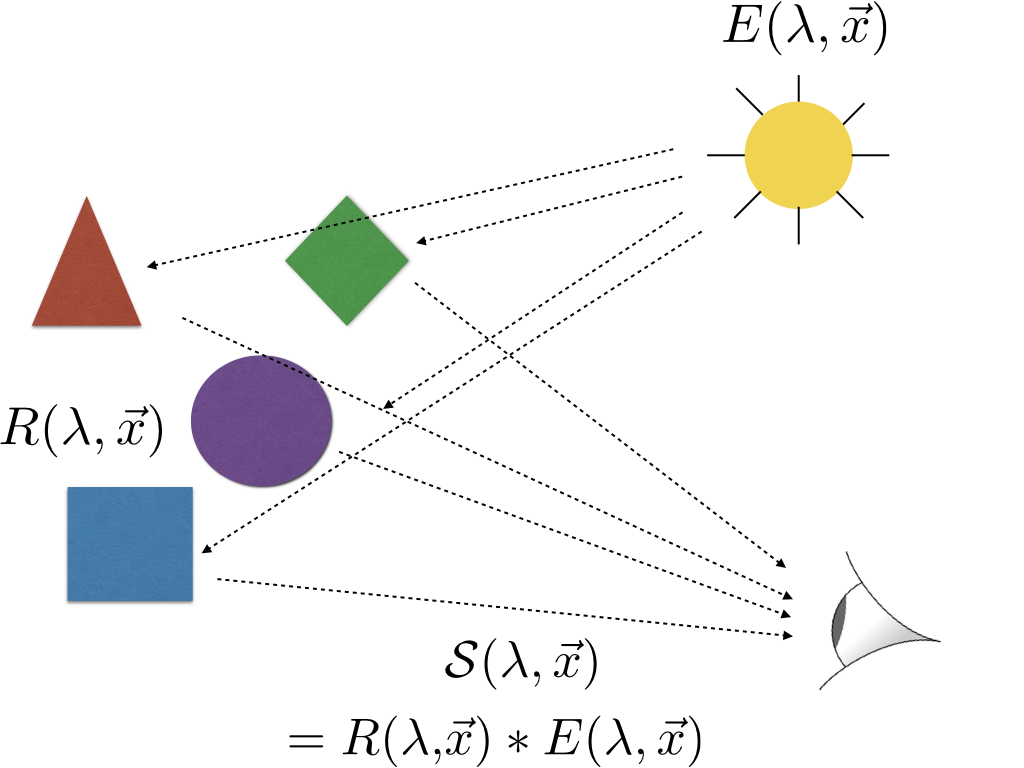
\includegraphics[width=\textwidth]{../Figures/Figure1/Figure1_a.png}
        \caption{}
        \label{fig:introSchematic}
    \end{subfigure}
    \begin{subfigure}{0.45 \textwidth}   
        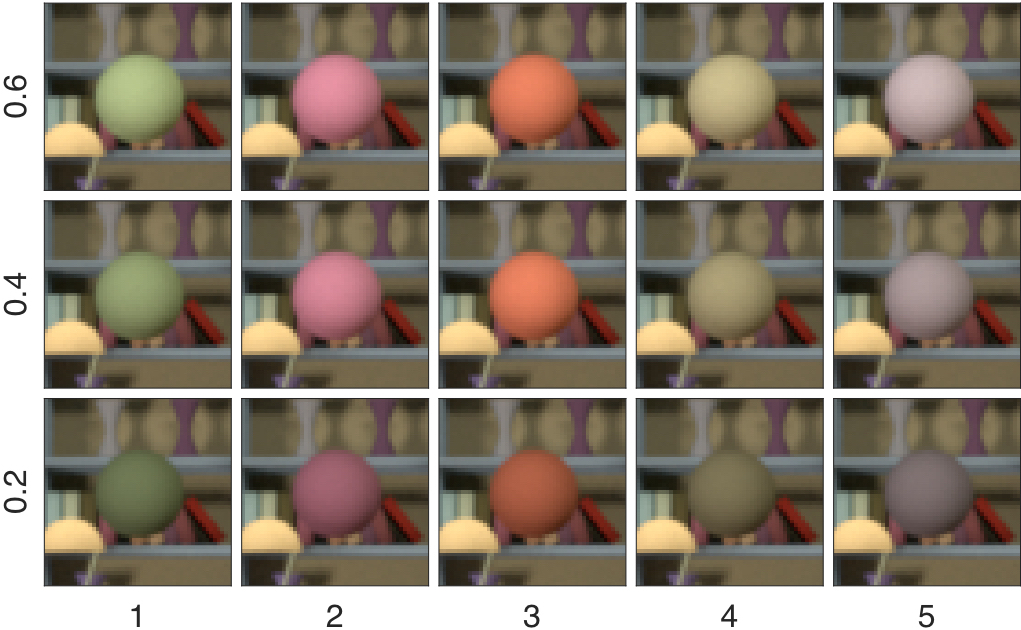
\includegraphics[width=\textwidth]{../Figures/Figure1/Figure1_b.jpeg}
        \caption{}
        \label{fig:introExampleFigure}
    \end{subfigure}
    \label{introFigure}
    \caption{(a) {\bf Color Constancy:} The light reflected from an object to our eyes depends both on the surface reflectance of the object, $R(\lambda,\vec{x})$, and the illumination spectrum of the light source, $E(\lambda,\vec{x})$. Additionally, it depends on geometric factors, such as the object's shape and pose, as well as the position of the observer. The human visual system is able to account for, at least partially, variations in the reflected light due to such extrinsic factors, and produce a percept of object color that is relatively stable with respect to such variations. Such invariant color perception is called color constancy. (b) {\bf Lightness Constancy Under Spectral Variations:} In this paper we consider the special case of lightness constancy. Fig.~\ref{fig:introExampleFigure} shows images of an object (the sphere in the center of each image) at three levels of object luminance. Within each row, the surface reflectance of the spheres has the same luminance, when illuminated by a standard reference illuminant, CIE D65. The three rows differ in this value, as can be seen by the fact that the lightness of the spheres generally decreases as we move down the columns. Within each row, the relative surface reflectance of the spheres varies, as can be seen by the variation in color appearance across the each row.  Within each column, this relative surface reflectance is held fixed. For illustration, we have kept the light source and the background obejcts fixed across the panels. See Fig.~\ref{fig:studiedCases} for images with such variations. In this paper, we seek to identify computations that accurately estimate object luminance across variations in relative surface reflectance, variations in illumination, and variation in the reflectance of other objects in the scene.}
 \end{figure}

The computational work reviewed above is based on formulating an explicit model of the image formation process and the statistical properties of natural images, and leveraging these formulations to obtain an appropriate ``inverse optics" algorithm.  An alternative approach, which has been less-well explored, is to use supervised machine learning techniques to develop mappings between input images and stable color descriptors.  Along these lines, Barron \cite{barron2015convolutional} recently developed a color balancing algorithm based on training a neural network to detect a uniform illuminant in an image by matching image templates in the chromaticity space. The use of supervised learning to understand human perceptual capabilities has enjoyed success in domains outside of color vision. Geisler and colleagues, for example, have developed a technique they refer to as accuracy maximization analysis (AMA, \citeNP{geisler2009optimal}), which learns linear filters whose output carries information that is optimized for particular perceptual tasks. This technique has provided computations that efficiently estimate speed \cite{burge2015optimal}, focus \cite{burge2011optimal} and disparity \cite{burge2014optimal} from image patches taken from natural scenes, and that in addition provide excellent models of human's ability to make corresponding estimates from the same stimuli.  In this paper, we apply AMA, as well as comparison supervised learning algorithms to a special case of the color constancy problem (lightness constancy) and evaluate how well it performs for naturalistic image input. 

A difficulty in using machine learning approaches for color constancy is that these approaches require large training sets with images of scenes containing objects with known surface reflectances illuminated with known illuminations.  Such data sets are not readily available. Although there are several databases of calibrated color natural images, these do not generally provide the corresponding information about surface and illuminant ground truth \cite{ChakrabartiHyperspectral,NascimentoFoster2016,ParragaHyperspectralData,TkacikUpennHypersepctralData,skauli2013collection},  ( ADD McGill Database). Generating databases with both the images and the ground truth scene information is not trivial. One approach has been to acquire mages where objects of known reflectance have been inserted into the scene, and to use the image of these reference objects to provide an estimate of the illumination impinging at various scene locations \cite{NascimentoFoster2016}.  This is somewhat painstaking, however, and in any case provides information about the illumination only at a small number of selected locations, so that generalizing across the image requires strong assumptions. Some progress is being made on characterizing how illumination varies over space in natural scenes \cite{mury2007spatial}, which in the longer run may guide how information from reference objects can be used to provide reasonable estimates.  Another approach is to acquire images of posed scenes, where the surface reflectances of objects are measured individually for many of the objects in the scene \cite{funt1988color,ciurea2003large} (ADD UCSB hyperspectral). These data sets have been useful for evaluating computational color constancy algorithms, but the use of posed scenes does not scale well for use with supervised learning methods which needs large training sets. 
 
% Figure 2: Cases Studied
\begin{figure}
\centering
	\begin{subfigure}[b]{0.33 \textwidth}
		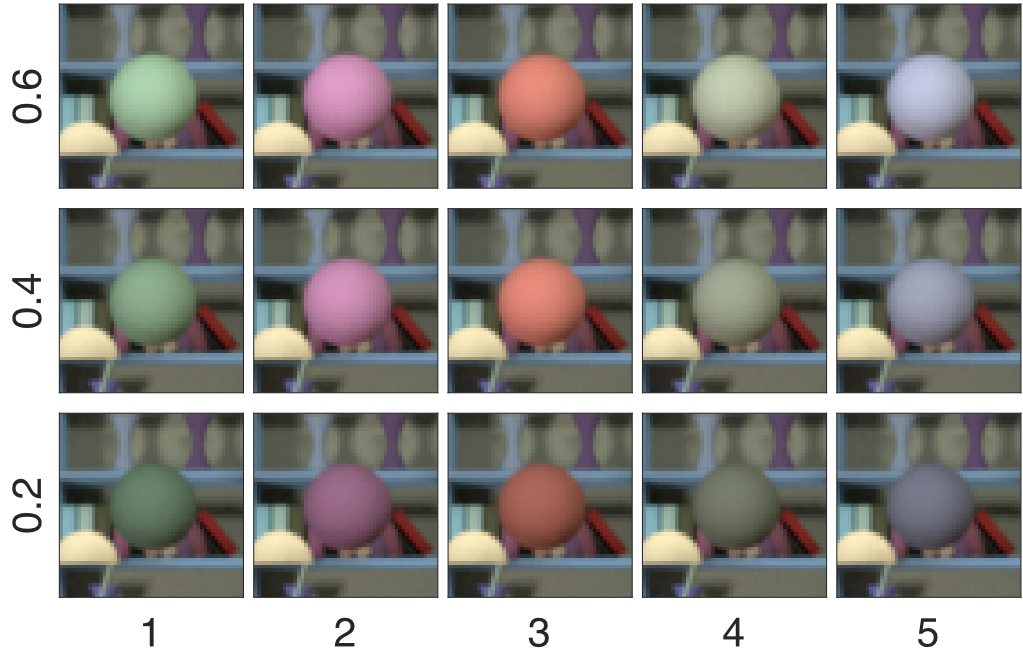
\includegraphics[width=\textwidth]{../Figures/Figure2/Figure2_a.jpeg}
		\caption{Case 1}
 		\label{fig:targetVarying}
	\end{subfigure}
	\begin{subfigure}[b]{0.33 \textwidth}
        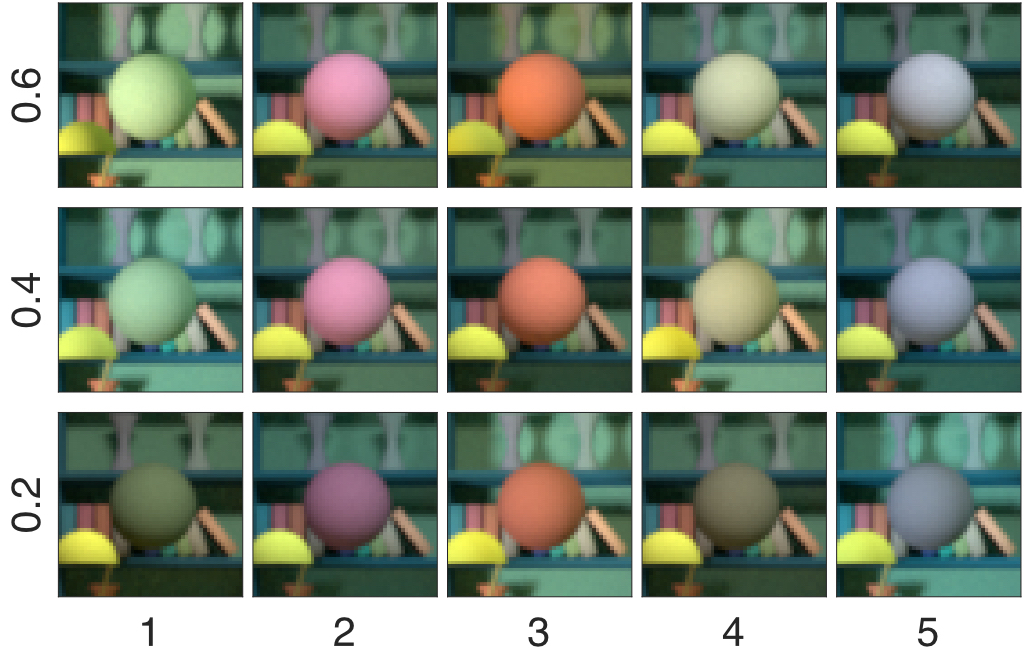
\includegraphics[width=\textwidth]{../Figures/Figure2/Figure2_b.jpeg}
        \caption{Case 2}
        \label{fig:targetIlluminantVarying}
    \end{subfigure}
	\begin{subfigure}[b]{0.33 \textwidth}
        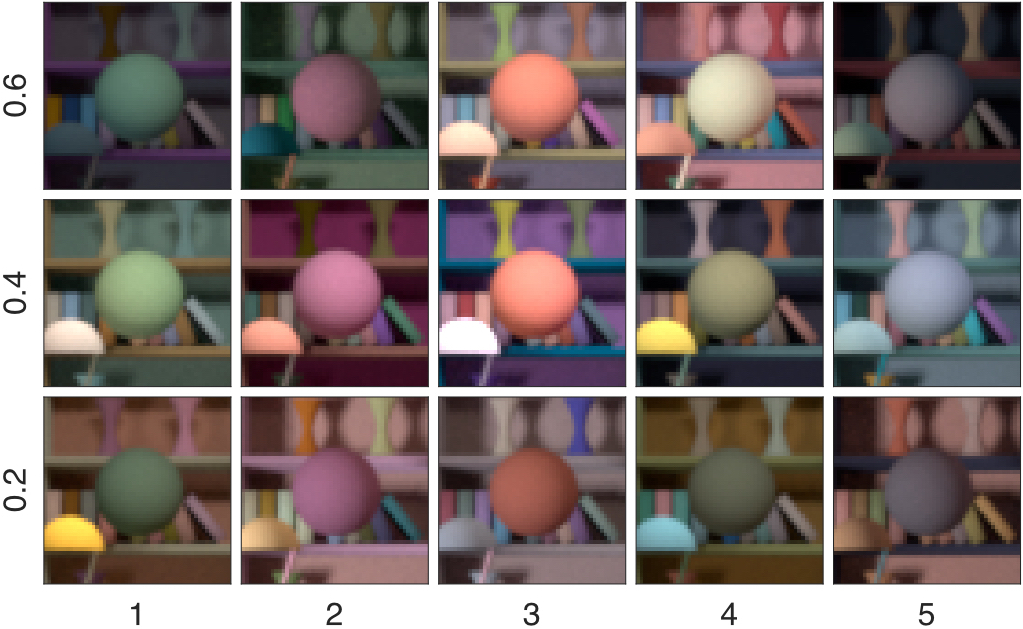
\includegraphics[width=\textwidth]{../Figures/Figure2/Figure2_c.jpeg}
        \caption{Case 3}
        \label{fig:allSpectraVarying}
    \end{subfigure}    
    \caption{{\bf Three types of spectral variations studied in this work:} sRGB rendition of multispectral images similar to ones studied in our work. The numbers on the left indicate the standard lightness level of the target object. 5 images are shown at each lightness level. We studied three types of spectral variations. (a) Case 1: target object relative surface reflectance spectrum variable, light source spectra fixed, background object spectra fixed, (b) Case 2: target object relative surface reflectance spectrum variable, light source spectra variable, background object spectra fixed, (c) Case 3: target object relative surface reflectance spectrum variable, light source spectra variable, background object spectra variable. This panel is reproduced from \ref{fig:introExampleFigure}. As in \ref{fig:introExampleFigure}, the spheres in each row of each panel have the same surface luminance, while the spheres in each column of each panel have the same relative surface reflectance.  Moreover, across the three panels of this figure, spheres in corresponding locations have the same surface reflectance. In all three panels, the overall lights source spectra scale factors (see \ref{Methods}) were drawn from a uniform distribution on the range [0.5, 1.5]. [CHECK THAT THIS WORKS FOR A NICE FIGURE].  The sRGB values for all three panels were normalized using a common scale factor prior to gamma correction.} 
\label{fig:studiedCases}
\end{figure}

Because of the difficulty in obtaining large labelled data sets of natural images for use in developing and evaluating computational color constancy algorithms, in this paper we adopt the approach of using high-quality computer graphics to render images of what we refer to as {\em virtual natural scenes}. Here, in addition to employing computer graphics to render the light reaching the eye from specified scenes, we also model the initial steps of the human visual system, so that our supervised learning methods are applied not to image pixels but rather to modeled responses of the foveal cone photoreceptor mosaic. We describe this approach in detail below, but the key advantage is that we can produce large numbers of naturalistic images and the corresponding cone mosaic responses, where all of the underlying scene properties are well-specified. This allows us to explore and evaluate computational color constancy with rich stimuli, while retaining the ability to precisely control and manipulate the intrinsic properties of the objects and illuminants that comprise the scene. This general approach has been adopted by other labs for the study of computational estimation of optical flow \cite{baker2011database} and is becoming increasingly popular (OTHER REFS: Cornell graphics person, Gallant, Yamins, Autonomous vehicle work), as well as for the generation of stimuli for the study of human perception (REFS: Many -- go to Boynton lecture slides for some).  Of course, success within the domain of graphics images does not guarantee smooth generalization to real natural images, a point we return to in the \nameref{Discussion}.

In this initial work, we do not tackle the full problem of color constancy.  Rather, as a point of departure, we consider the computational problem of estimating a single attribute of object surface reflectance, which we refer to as surface luminance.  We compute object luminance from an object's surface reflectance function as follows.  We compute the light that would be reflected to the eye from a flat matte object with that surface reflectance, when the object is diffusely illuminated by the standard CIE daylight spectrum D65 \cite{CIE86}.  We then compute the luminance of this reflected light, using the CIE 1931 photopic luminosity function \cite{CIE86}, and divide this by the luminance of a perfectly reflecting diffuser (surface reflectance of one at all wavelengths) when that is computed in the same way. This procedure allows us to assign to any surface reflectance a single surface luminance value.  Because the perceived lightness of an object is approximately (but by no means exactly, see \citeNP{wyszecki1986color}) correlated with surface luminance across a range of viewing conditions, we refer to the computational problem we study as that of {\em lightness constancy}.
This is a generalization of the way this term is often used, where it refers more specifically to the stability of perceived lightness across images of scenes where all objects and illuminants are achromatic \cite{gilchrist2006seeing}.
Here, we aim to estimate surface luminance, but do so for images where both the luminance and the chromaticity of the surfaces and illuminants varies (see  Fig.~\ref{fig:introExampleFigure}). A particularly important feature of our treatment is that we consider scene variations where not only the spectrum of the illumination varies, but also the surface reflectance of objects in the scene other than the object whose surface luminance is being estimated. 

Even within the special case of lightness constancy, there are many scene manipulations that could be considered. The set of manipulations we focus on here are illustrated by the three panels of Fig.~\ref{fig:studiedCases}. These cases are: 1. variation in target object spectrum with fixed light source and background objects spectra (Fig.~\ref{fig:targetVarying}), 2. variations in both the target object spectrum and the light source spectra, with fixed background object spectra (Fig.~\ref{fig:targetIlluminantVarying}), and 3. variations in all three types of spectra (target object, light source, and background objects) (Fig.~\ref{fig:allSpectraVarying}). Across real scenes, there will also be variations in the shape of the target object, its pose, eye position, etc. (see \nameref{Methods}). In this paper, we focus on the problem of lightness constancy within scene ensembles where these geometric factors are held fixed.

We show that for cases that have spectral variation only either in target object surface reflectance or background object surface reflectance or the power spectrum of the light sources, lightness can be estimated by simple transformations of the cone responses. For variations only in target object reflectance spectra (case 1), object lightness can be recovered directly from the light reflected off the target object. For case 2, where both the target object reflectance and light source spectra vary, object lightness can be recovered from the contrast between the target and the background. When all the spectral features in the scene are allowed to change (case 3), the standard lightness can not be recovered simply from the cone response or the contrast. Here, we have used two supervised learning methods with Bayesian estimators to estimate standard lightness of the target object. Using these methods, we can recover the lightness of the target object with $\sim 15\%$ relative root mean square error.  Our analysis shows that the optimal receptive fields for estimating the lightness of the target object show a center surround structure, supporting a comparison between the light coming from the target object and its surround. Additionally, lightness estimation involves a weighted sum of the L, M and S cone responses where the receptive fields give more weight to the L and M cone responses compared to S cone responses. Comparing the performance of the RFs learnt using  one case on the cone response of other cases shows that the receptive field of the complex cases perform well on images of simpler cases. We discuss the implications of such receptive fields on lightness constancy. 

The rest of this paper is organized as follows. In the \nameref{Methods} section, we describe in detail the process to generate naturalistic labeled images (\nameref{method:VirtualWorld}) using our software pipeline {\rm Virtual world color constancy}, the process to simulate the response of retinal cone photoreceptors to these images using a standard model of the early visual system (\nameref{method:Isetbio}) and the supervised learning methods used in our analysis (\nameref{method:SupervisedLearning}). In the \nameref{Results} section, we show the estimates and performance of the supervised methods for the three cases mentioned above. We conclude the paper with the implication of our results in the \nameref{Discussion} section.  

\section*{Methods} \label{Methods}
\subsection{Overview}
There are four key parts to our methods.  The first is how we generate a labelled set of training data for our supervised learning algorithms.  The second is how we model the transformations applied by the early visual system to generate modeled responses of the cone photoreceptor mosaic.  The third is the details of the supervised learning methods we apply to the labelled training data.  And the fourth is how we evaluate the performance of the algorithms.  We describe each of these in the sections below.

\subsection{Labelled image database} \label{method:VirtualWorld}

\subsubsection{Virtual naturalistic scenes}
The light that reflects off an object and reaches our eyes depends on many factors. These factors include: the surface reflectance of the object, the surface reflectance, texture, material and geometry of the objects in its surround, the spectrum of the sources of light illuminating the object, and the position of the observer. In natural scenes, these spectral and geometrical factors vary considerably. To study the effect of these factors on color perception, we need a system that can generate natural scenes with precise control over all such factors. We need a system that can produce natural scenes at a fixed perceived color of a target object, while having a representative, but precisely quantified, sampling of the variations in the scene. Under natural conditions it is difficult to control and quantify every such parameter in a scene. Thus generating such a dataset, with a representative sampling of natural variations, is considerably time and labor intensive.

To overcome this  challenge, we have developed an image rendering software pipeline that allows us to specify a virtual, but naturalistic, statistical model of visual scenes with parametric control over factors in natural scenes. The software uses a physically-based image rendering system that accurately accounts for the interactions of light with matter in 3D scenes. It then renders a multispectral 2D image of each modeled visual scene. Wherever possible, we have incorporated statistical models of the variation of specific scene parameters based on observed data in natural scenes. In addition, our software simulates the responses of retinal cones to the rendered multispectral images using a realistic model of the early human visual system. Below we provide the details of the software and the choices made to generate ensembles of scenes with corresponding images. Our software, which is written in MATLAB, is freely available through a public respository: \href{https://github.com/BrainardLab/VirtualWorldColorConstancy}{Virtual World Color Constancy}. It builds on several other open source projects, including \href{http://rendertoolbox.org}{RenderToolbox4} \cite{heasly2014rendertoolbox3}, \href{http://isetbio.org}{Isetbio} and \href{https://www.mitsuba-renderer.org}{Mitsuba} \cite{jakob2015mitsuba}. Below we refer to the software pipeline as VWCC (for Virtual World Color Constancy).

The process of generating an individual virtual scene begins with the selection of a \textit{base scene} (Fig.~\ref{fig:baseScenes}). The base scene is a 3D model that defines a rendering space.  It typically includes the specification of a number of 3D objects and light sources, and is annotated with meta-data that may be used to guide the placement of additional objects and light sources, as well as the specification of camera position. VWCC includes a library of base scenes obtained from materials made available on the Internet under various Creative Commons licenses. We have found that there is sufficient variation in how nominally-standard graphics interchange file formats are used in practice that each base scene obtained from the Internet (which we refer to as \textit{wild scenes}) requires a certain amount of hand editing before it renders properly. We refer to this process, along with adding meta-data about the scene, as \textit{taming} a wild scene. Tame base scenes may also be created de novo using a 3D modeling software (e.g., \href{https://www.blender.org/}{Blender}).  The overall spatial scale of the base scene may be adjusted under programmatic control or chosen randomly, adding to the available statistical richness. If one chooses to draw entries from the base scene library at random for each virtual scene, the base scene library then provides a simple statistical model of the gross layout of natural scenes. As time progresses, we plan to tame more wild scenes so as to increase the number of entries in the base scene library. Currently the library contains 6 base scenes: Library (Fig.~\ref{fig:baseSceneLibrary}), Mill (Fig.~\ref{fig:baseSceneMill}), Table-Chairs (Fig.~\ref{fig:baseSceneTableChairs}), Indoor plant (Fig.~\ref{fig:baseSceneIndoorPlant}), Checkerboard (Fig.~\ref{fig:baseSceneWarehouse}) and Warehouse (Fig.~\ref{fig:baseSceneCheckerBoard}).

% Figure 3
\begin{figure}[t]
\centering
\begin{subfigure}[b]{0.22 \textwidth}
        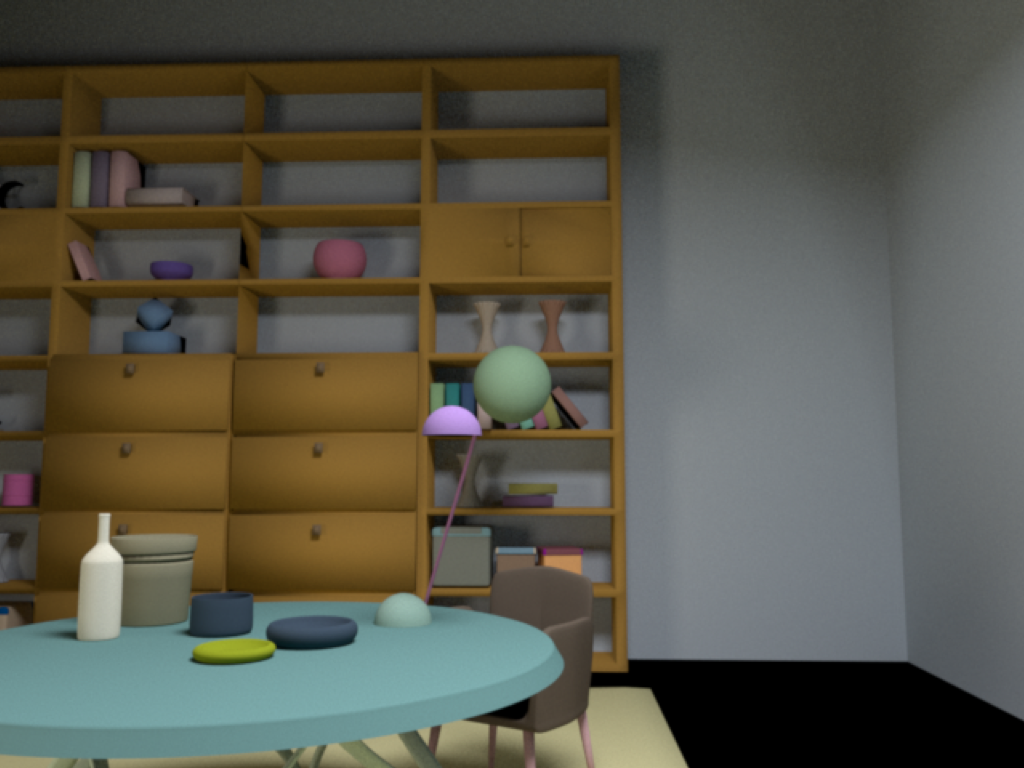
\includegraphics[width=\textwidth]{../Figures/Figure3/Figure3_a.png}
        \caption{Library }
        \label{fig:baseSceneLibrary}
    \end{subfigure}
    ~ %add desired spacing between images, e. g. ~, \quad, \qquad, \hfill etc. 
      %(or a blank line to force the subfigure onto a new line)
    \begin{subfigure}[b]{0.22 \textwidth}
        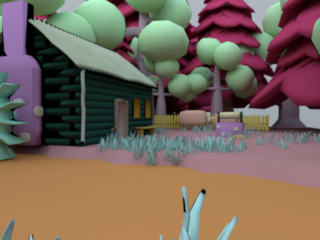
\includegraphics[width=\textwidth]{../Figures/Figure3/Figure3_b.png}
        \caption{Mill}
        \label{fig:baseSceneMill}
    \end{subfigure}    
    ~ %add desired spacing between images, e. g. ~, \quad, \qquad, \hfill etc. 
    %(or a blank line to force the subfigure onto a new line)
    \begin{subfigure}[b]{0.22 \textwidth}
        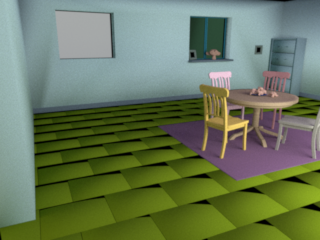
\includegraphics[width=\textwidth]{../Figures/Figure3/Figure3_c.png}
        \caption{Table-Chairs}
        \label{fig:baseSceneTableChairs}
    \end{subfigure}
    
    \begin{subfigure}[b]{0.22 \textwidth}
        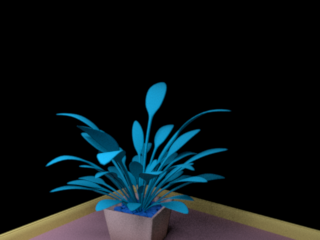
\includegraphics[width=\textwidth]{../Figures/Figure3/Figure3_d.png}
        \caption{Indoor-plant}
        \label{fig:baseSceneIndoorPlant}
    \end{subfigure}    
    ~
    \begin{subfigure}[b]{0.22 \textwidth}
        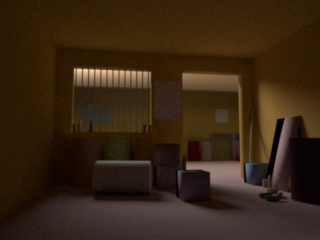
\includegraphics[width=\textwidth]{../Figures/Figure3/Figure3_e.png}
        \caption{Warehouse}
        \label{fig:baseSceneWarehouse}
    \end{subfigure}
    ~
    \begin{subfigure}[b]{0.22 \textwidth}
        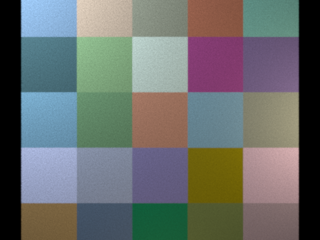
\includegraphics[width=\textwidth]{../Figures/Figure3/Figure3_f.png}
        \caption{Checkerboard}
        \label{fig:baseSceneCheckerBoard}
    \end{subfigure}
    \caption{{\bf Example of base scenes form the VWCC library.} Each panel shows a rendering of one tamed base scene without additional objects inserted.  The reflectance spectra of the distinct surfaces in each scene has been assigned randomly (see below) using the VWCC software.  The light source spectra were also assigned randomly to the default and inserted light source.}\label{fig:baseScenes}
\end{figure}

VWCC provides an option for inserting 3D objects and lights sources into the base scene. Fig.~\ref{fig:libraryWithTarget} shows examples of objects inserted into the library base scene. The object shapes may be selected from a VWCC library that, similar to the VWCC library of base scenes, has been tamed from object descriptions made available on the Internet. The light sources may be chosen as point lights, area lights, or as shapes selected from the object library. The position (Fig.~\ref{fig:targetPositionVariation}), size and orientation (Fig.~\ref{fig:targetSizeOrientation})of the inserted objects and lights may be specified programatically or chosen randomly under constraints provided by the base scene meta-data. Thus, along with distributions that characterize parameters such as the number, size, shape and orientation of the inserted objects and light sources, we have a simple statistical model of the object and light source geometry of natural scenes. 

% Figure 4
\begin{figure}[h]
\centering
\begin{subfigure}[b]{0.14 \textwidth}
        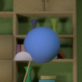
\includegraphics[width=\textwidth]{../Figures/Figure4/Figure4_a.png}
        \caption{Big-ball}
        \label{fig:libraryWithBigBall}
    \end{subfigure}
    ~ %add desired spacing between images, e. g. ~, \quad, \qquad, \hfill etc. 
      %(or a blank line to force the subfigure onto a new line)
\begin{subfigure}[b]{0.14 \textwidth}
        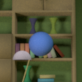
\includegraphics[width=\textwidth]{../Figures/Figure4/Figure4_b.png}
        \caption{Small-ball}
        \label{fig:libraryWithSmallBall}
    \end{subfigure}
    ~ %add desired spacing between images, e. g. ~, \quad, \qquad, \hfill etc. 
      %(or a blank line to force the subfigure onto a new line)
    \begin{subfigure}[b]{0.14 \textwidth}
        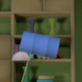
\includegraphics[width=\textwidth]{../Figures/Figure4/Figure4_c.png}
        \caption{Barrel}
        \label{fig:libraryWithBarrel}
    \end{subfigure}
    \begin{subfigure}[b]{0.14 \textwidth}
        
\includegraphics[width=\textwidth]{../Figures/Figure4/Figure4_d.png}
        \caption{Xylophone}
        \label{fig:libraryWithXylophone}
    \end{subfigure}
    ~
	\begin{subfigure}[b]{0.14 \textwidth}
        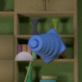
\includegraphics[width=\textwidth]{../Figures/Figure4/Figure4_e.png}
        \caption{Ring toy}
        \label{fig:libraryWithRingToy}
    \end{subfigure}
        ~
    	\begin{subfigure}[b]{0.14 \textwidth}
        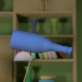
\includegraphics[width=\textwidth]{../Figures/Figure4/Figure4_f.png}
        \caption{Bottle}
        \label{fig:libraryWithChampagneBottle}
    \end{subfigure}
\caption{{\bf Library base scene with inserted objects.} The VWCC software was used to insert different objects into the library base scene, with each panel showing a different object. The objects were inserted at a location in the image and then the camera was pointed at the object, so that the object's image is at the center of the rendered image.  In the figure panels, the full rendered image is cropped so that the inserted object is more visually salient. We use this capability of our software pipeline to insert target objects into scenes.}\label{fig:libraryWithTarget}
\end{figure}

% Figure5
\begin{figure}
\centering
	\begin{subfigure}[b]{0.18 \textwidth}
    \centering
        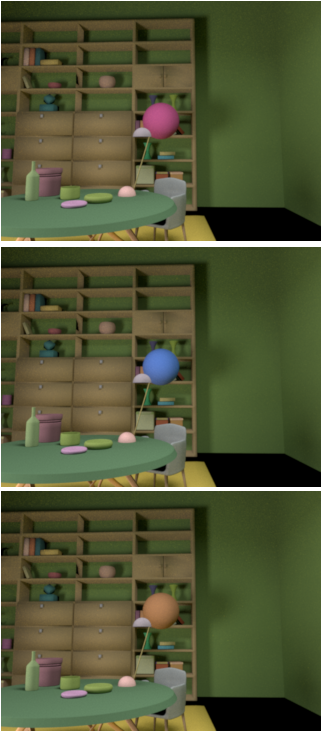
\includegraphics[width=\textwidth]{../Figures/Figure5/Figure5_a.png}
        \caption{Target spectra}
        \label{fig:targetVariation}
    \end{subfigure}
    ~ %add desired spacing between images, e. g. ~, \quad, \qquad, \hfill etc. 
      %(or a blank line to force the subfigure onto a new line)
    \begin{subfigure}[b]{0.18 \textwidth}
    \centering
        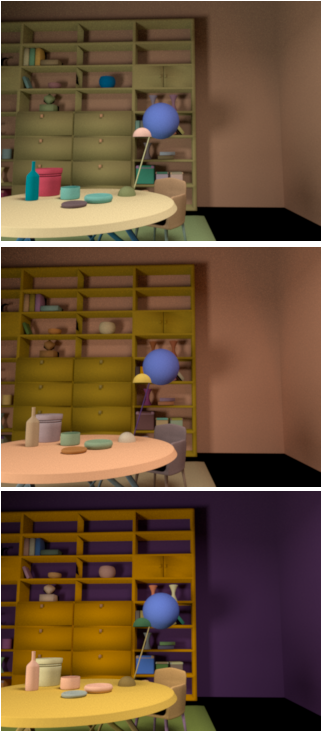
\includegraphics[width=\textwidth]{../Figures/Figure5/Figure5_b.png}
        \caption{Background spectra}
        \label{fig:backGroundVariation}
    \end{subfigure}
    ~ %add desired spacing between images, e. g. ~, \quad, \qquad, \hfill etc. 
    %(or a blank line to force the subfigure onto a new line)
    \begin{subfigure}[b]{0.18 \textwidth}
    \centering
        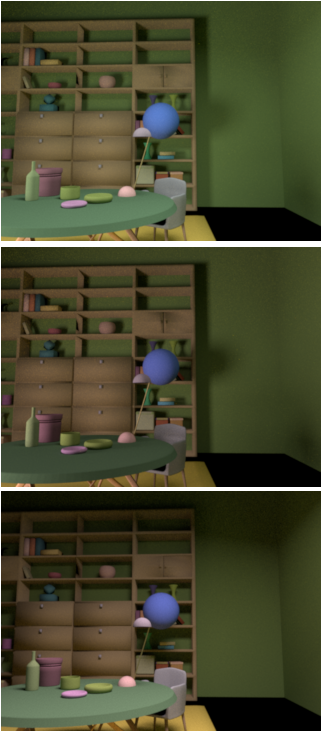
\includegraphics[width=\textwidth]{../Figures/Figure5/Figure5_c.png}
        \caption{Illumination spectra}
        \label{fig:illuminationVariation}
    \end{subfigure}
    ~ %add desired spacing between images, e. g. ~, \quad, \qquad, \hfill etc. 
      %(or a blank line to force the subfigure onto a new line)
	\begin{subfigure}[b]{0.18 \textwidth}
    \centering
        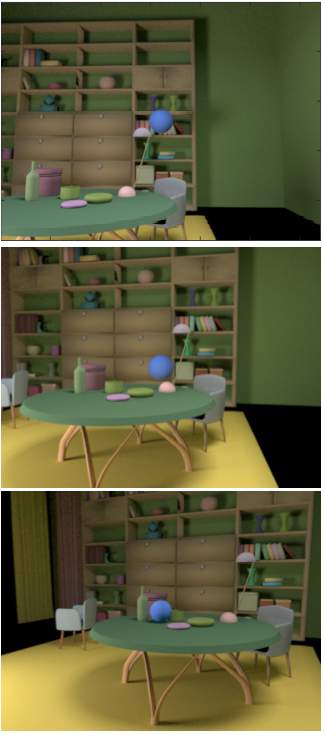
\includegraphics[width=\textwidth]{../Figures/Figure5/Figure5_d.png}
        \caption{Target position}
        \label{fig:targetPositionVariation}
    \end{subfigure}
    ~ %add desired spacing between images, e. g. ~, \quad, \qquad, \hfill etc. 
      %(or a blank line to force the subfigure onto a new line)
	\begin{subfigure}[b]{0.18 \textwidth}
    \centering
        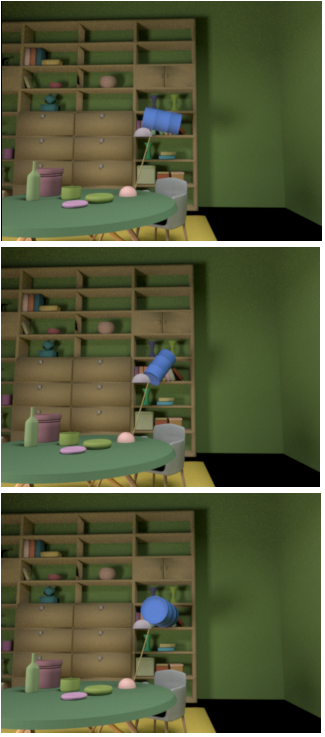
\includegraphics[width=\textwidth]{../Figures/Figure5/Figure5_e.png}
        \caption{Target Size/Orientation}
        \label{fig:targetSizeOrientation}
    \end{subfigure}
    ~ %add desired spacing between images, e. g. ~, \quad, \qquad, \hfill etc. 
      %(or a blank line to force the subfigure onto a new line)
    \caption{{\bf Transformations of the scene.} The possible transformations of the properties of a scene can broadly be classified into two groups: Spectral (a-c) and Geometrical (d-e). VWCC provides control over such transformation as illustrated by the columns. (a) The target object surface reflectance varies across the three panels of the column. (b) The surface reflectance of the background objects varies across the three panels. In each panel, the reflectances were assigned randomly. (c) The power spectrum of the light sources were assigned randomly in the three panels. (d) The three panels in the column have the target object at three different positions. The camera points to the center of the pixel. }\label{fig:VWCCTransformations}
\end{figure}

Once a base scene has been chosen and objects and light sources inserted, we assign spectral surface reflectance, texture, and material property to each object surface in the scene. We also assign an illuminant spectral power distribution to each light source in the scene. Objects in the VWCC library may contain more than one distinct surface, each of which may be assigned a different surface reflectance. As with object position, these may be specified programatically. In the present work, we use simple choices for texture (all surfaces spatially uniform) and material property (all surfaces matte) and focus on variation in surface spectral reflectance. 

In the present work, we insert one target object and one additional light source into a fixed base scene, and vary reflectance and illuminant spectra. We then insert a camera for rendering at a user specified position and point this camera at the target object. We ensure that a 9 pixel by 9 pixel region at the center of the image corresponds to light reflected from the target object, which amounts to verifying that the target object at its inserted position was not occluded by other objects in the line of sight from camera. For each rendered scene, we specify the surface reflectance of the target object, which allows us to control both its surface luminance as well as its relative surface reflectance. The specified surface luminance provides the requisite label for the scene and resultant cone mosaic responses.

We render scenes using the \href{https://www.mitsuba-renderer.org}{Mitsuba} \cite{jakob2015mitsuba} rendering package, driven by our \href{http://rendertoolbox.org}{RenderToolbox4} \cite{heasly2014rendertoolbox3} rendering pipeline.

For the images used for the primary results reported in this paper, we used the ``{\it Library}'' base scene from the VWCC  and the ``{\it Big Ball}'' object as the target object. We also inserted a spherical light source with the same ``{\it Big Ball}'' shape. The position, and size of the inserted object, light source and the camera were held fixed for all the images analyzed in this work, i.e., the scene geometry did not vary. Next, we assigned illumination and surface reflectance spectra to the lights and objects in the scene. The spectral manipulations for the various cases studied in this work have been described in the main text (Fig.~\ref{fig:studiedCases}). 2D multispectral images were rendered at 31 wavelengths from $400$nm to $700$nm spaced $10$nm apart at an image size $320\times 240$ pixel$^2$. A $51 \times 51$ pixel$^2$ patch of the multispectral image was cropped around the target object and cone responses were calculated to these cropped images. 

[GOT TO HERE]
\subsubsection{Illumination Spectra}
The illumination spectrum is generated through a random statistical sampling of a natural illumination spectrum dataset. First, we approximate the spectra in the dataset using principle component analysis (PCA). We decompose the spectra as a linear sum over the PCA basis vectors corresponding to the largest 6 PCA eigenvalues. Next, we sample random spectra from this low 6 dimensional PCA space assuming the spectral distribution to be a multivariate gaussian.

% Figure 6
\begin{figure}
\centering
	\begin{subfigure}[b]{0.3 \textwidth}
    \centering
        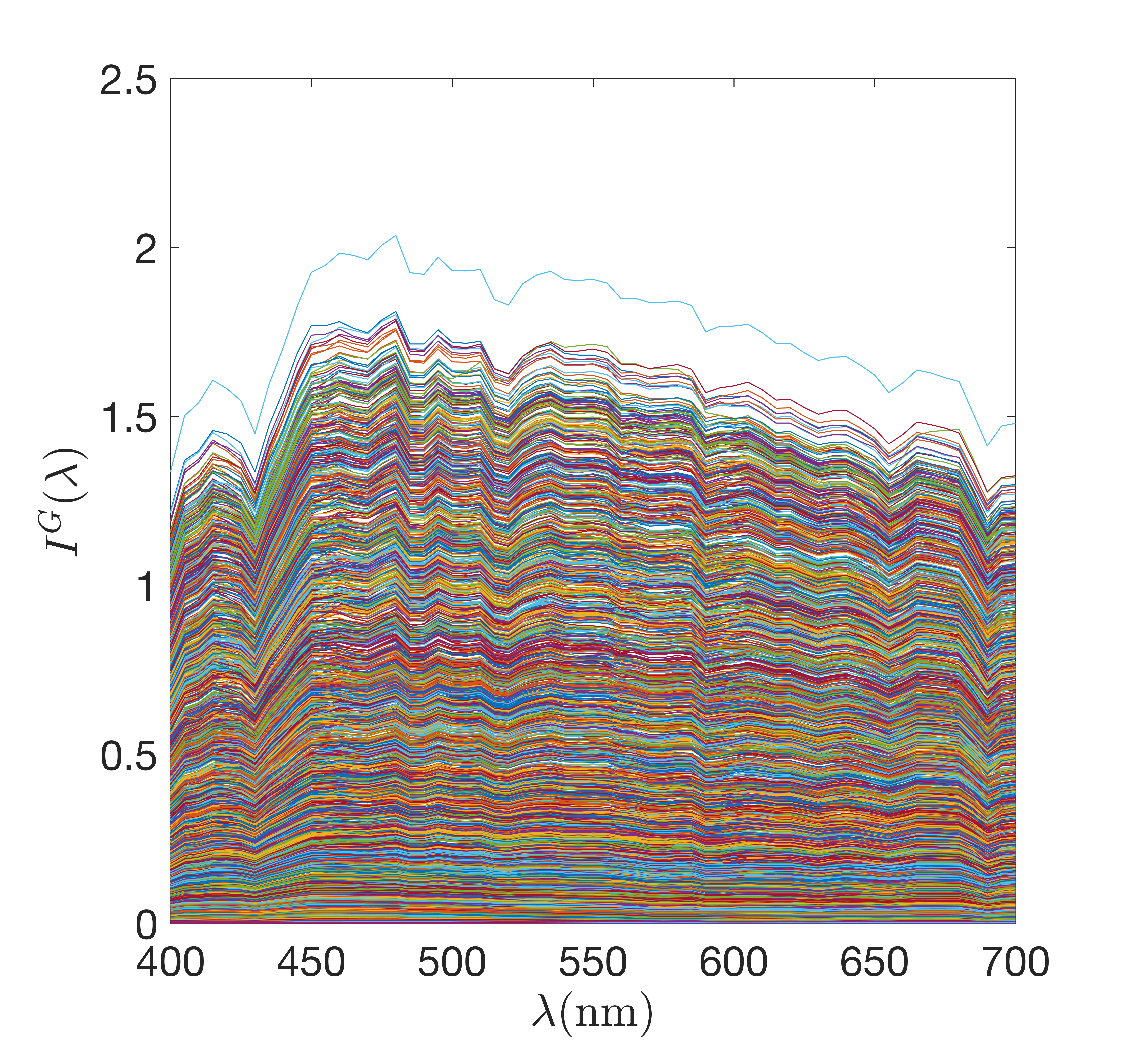
\includegraphics[width=\textwidth]{../Figures/Figure6/Figure6_a.pdf}
        \caption{Granada natural daylight dataset}
        \label{fig:granadaSpectra}
    \end{subfigure}
    \begin{subfigure}[b]{0.3\textwidth}
    \centering
        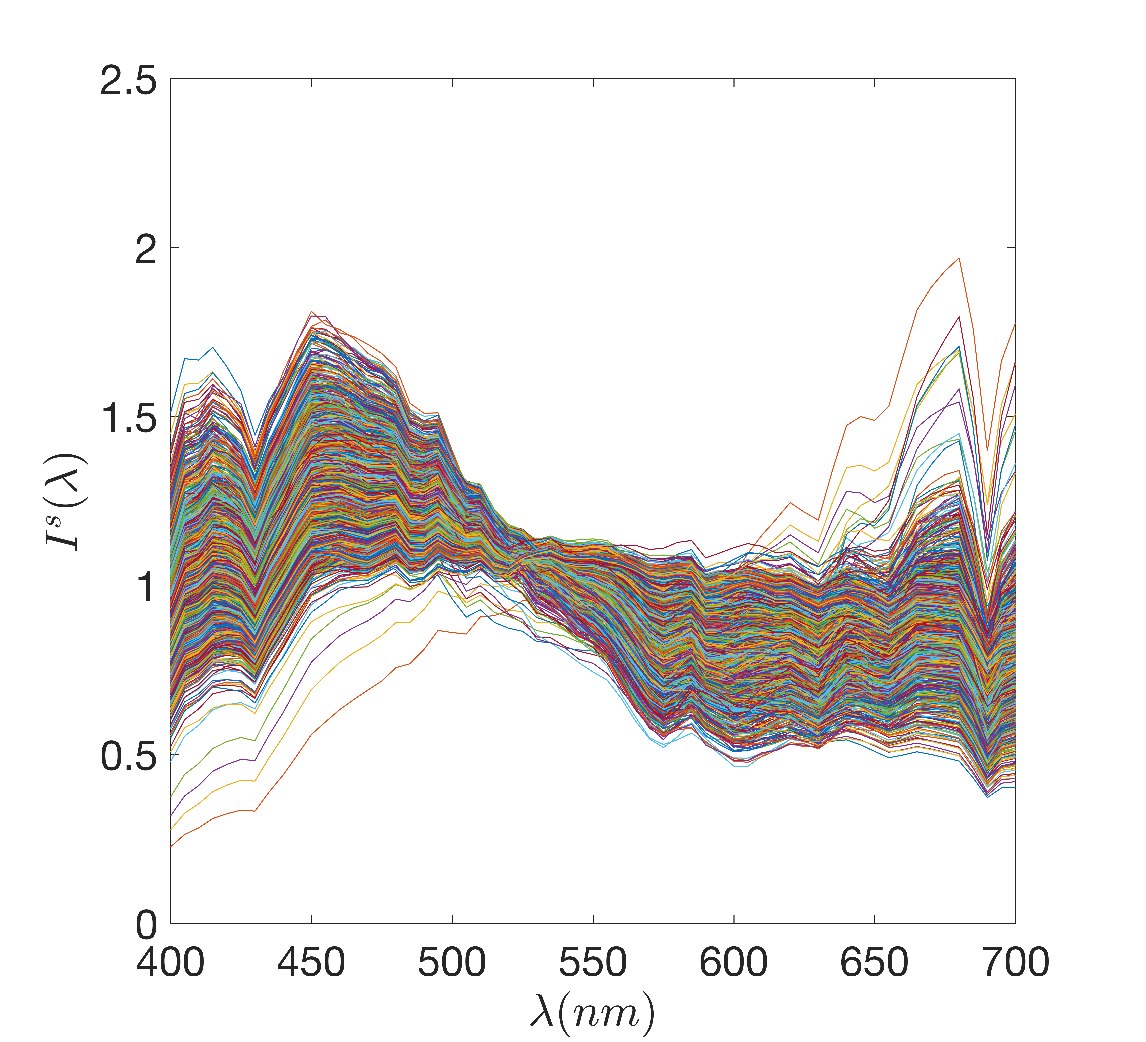
\includegraphics[width=\textwidth]{../Figures/Figure6/Figure6_b.pdf}
        \caption{Rescaled Granada dataset}
        \label{fig:rescaledGranada}
    \end{subfigure}
    \begin{subfigure}[b]{0.3 \textwidth}
    \centering
        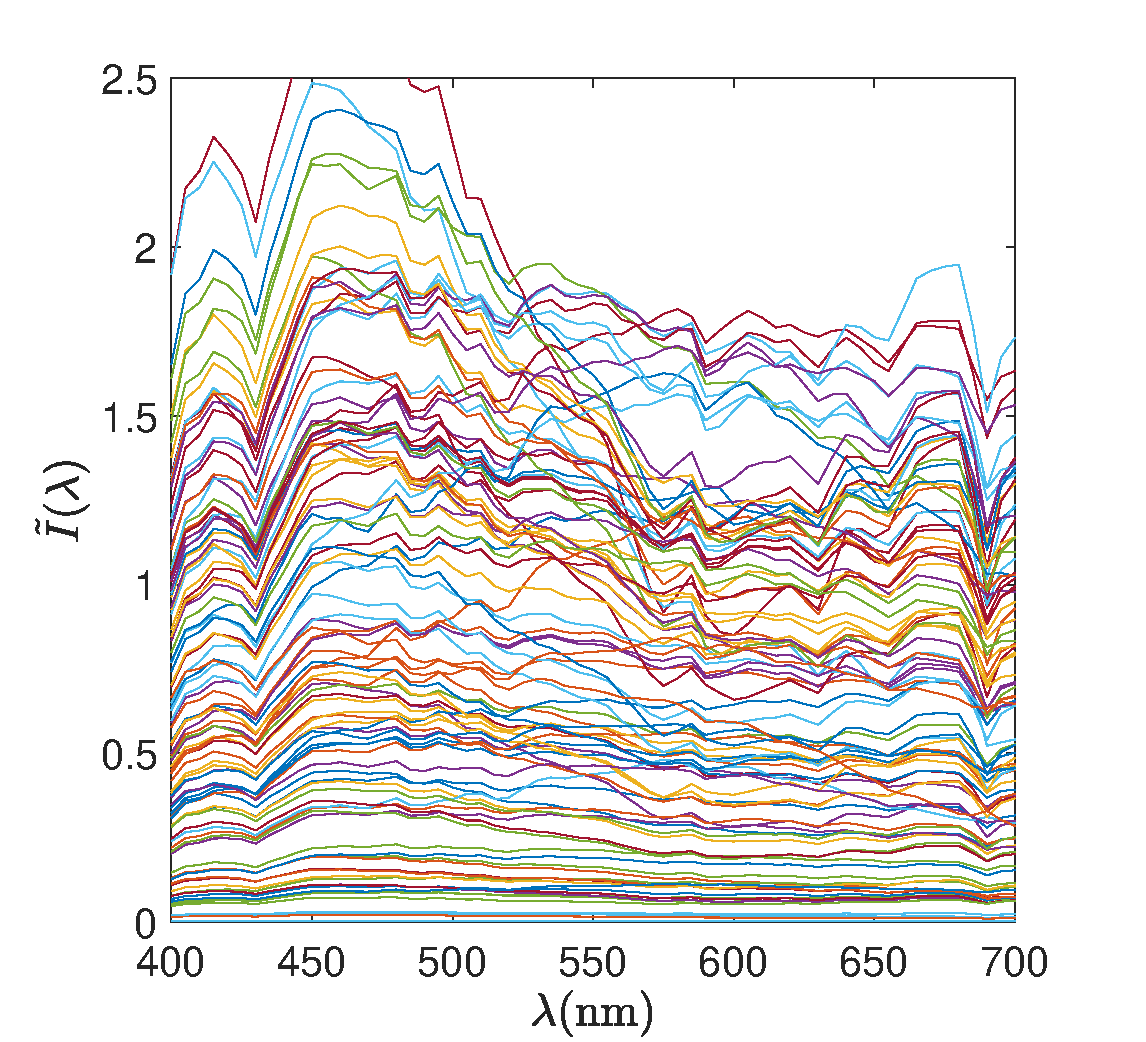
\includegraphics[width=\textwidth]{../Figures/Figure6/Figure6_c.pdf}
        \caption{Randomly generated samples}
        \label{fig:randomIlluminant}
    \end{subfigure}

	\begin{subfigure}[b]{0.3 \textwidth}
    \centering
        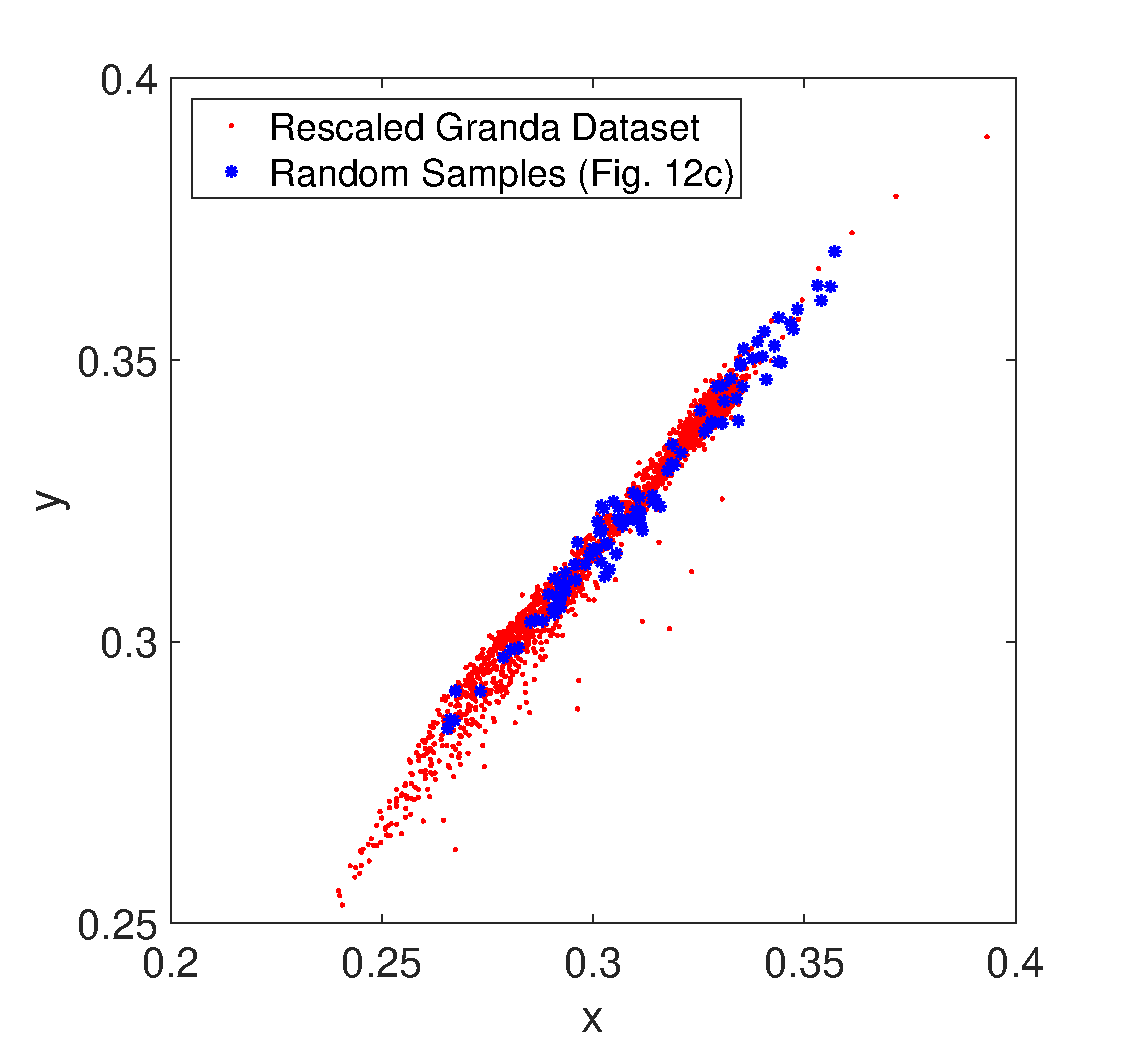
\includegraphics[width=\textwidth]{../Figures/Figure6/Figure6_d.pdf}
        \caption{xy chromaticity diagram}
        \label{fig:xyDiagram}
    \end{subfigure}
	\begin{subfigure}[b]{0.3 \textwidth}
    \centering
        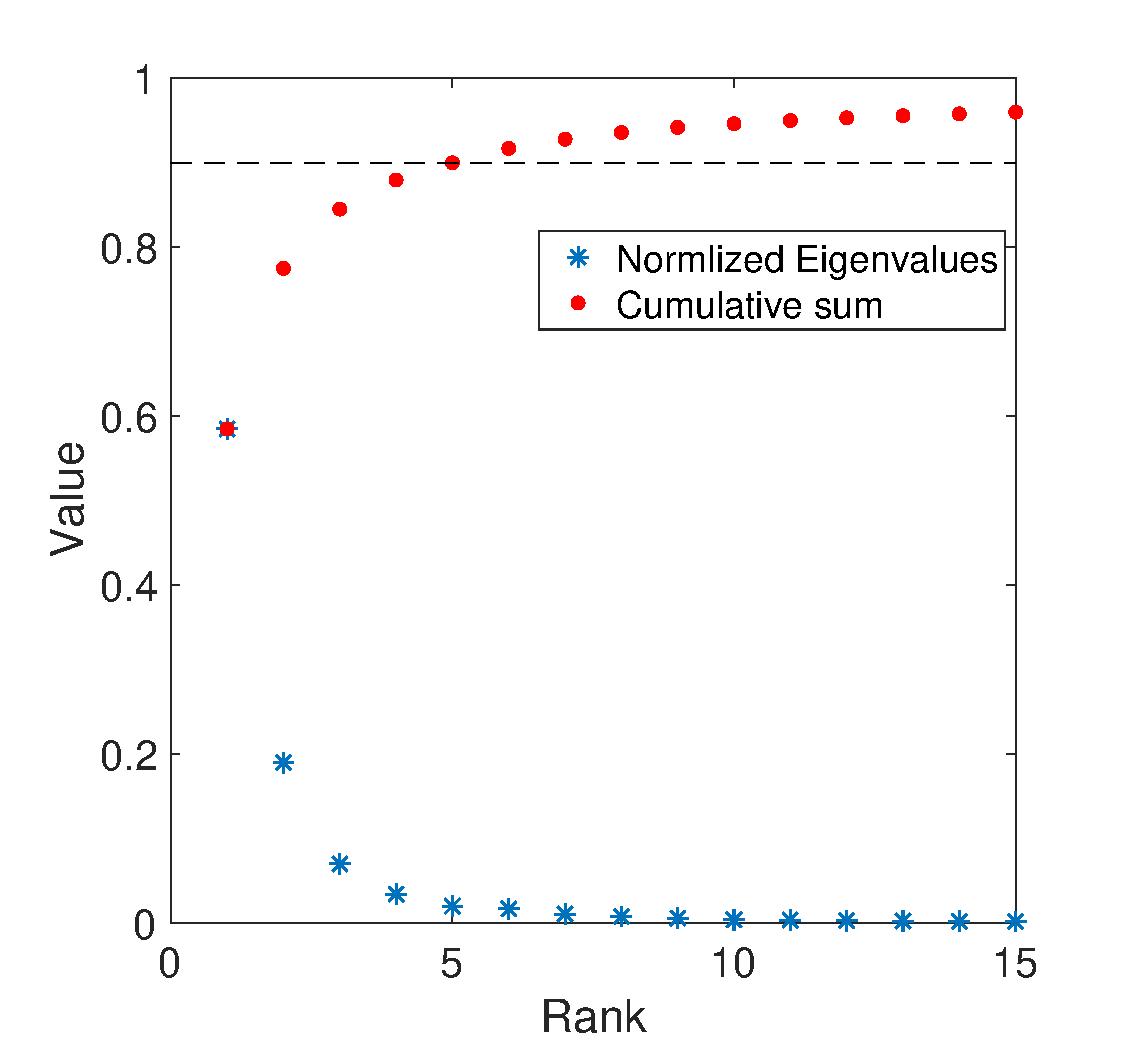
\includegraphics[width=\textwidth]{../Figures/Figure6/Figure6_e.pdf}
        \caption{Normalized PCA eigenvalues}
        \label{fig:granadaEV}
    \end{subfigure}
      	\begin{subfigure}[b]{0.3 \textwidth}
    \centering
        
\includegraphics[width=\textwidth]{../Figures/Figure6/Figure6_f.pdf}
        \caption{sRGB rendition of samples from Fig.\ref{fig:randomIlluminant}}
        \label{fig:sRGBIlluminant}
    \end{subfigure}
    \caption{{\bf Generating random illumination spectrum:} The illumination spectra are generated by random sampling of Granada daylight spectra assuming a multivariate gaussian distribution. The mean and variance of the gaussian are chosen by projecting the dataset along PCA directions and taking the mean and covariance of the projections. (a) Granada natural daylight dataset. (b) Rescaled Granada dataset. Each spectra is rescaled by its mean illumination over frequency. (c) Randomly generated samples. (d) xy chromaticity diagram of the rescaled dataset (Fig. \ref{fig:rescaledGranada}) and the randomly generated samples (Fig.\ref{fig:randomIlluminant}). (e) Normalized PCA eigenvalues and cumulative sum of the normalized eigenvalues. The eigenvalues have been normalized by the sum over all eigenvalues. The dotted line (= 0.9) is for reference. We choose the first six eigenvectors in ur analysis. (f) The sRGB renditions of the random samples generated in \ref{fig:randomIlluminant}.}\label{fig:illluminationGeneration}
\end{figure}

We have used the Granada natural daylight spectrum \href{http://colorimaginglab.ugr.es/pages/Data}{dataset} \cite{peyvandi2016colorimetric} to sample illuminants. Let us denote the Granada dataset as $I^G_i(\lambda)$, where $\{i \in [1,M]\}$ and $M$ is the total number of spectra in the dataset. Since the distribution varies over multiple order of magnitudes, we rescale each spectrum by dividing by its mean $I_i^s(\lambda) = \frac{I^G_i(\lambda)}{\int d\lambda I^G_i(\lambda)}$. These rescaled spectra $(I_i^s(\lambda))$ are then mean centered for PCA by subtracting out the mean 
rescaled spectra, $\bar{I}^{s}(\lambda)$. The mean is obtained
by taking the sample mean over all spectra in the dataset, $\bar{I}^{s}(\lambda) = \frac{1}{M}\sum_i{I_i^s(\lambda)}$. 
The resulting mean subtracted dataset, $I_i^{MC}(\lambda) = I_{s}(\lambda) - \bar{I}_{s}(\lambda)$, 
is decomposed as $I_i^{MC}(\lambda) = \sum_j w_{ij}\hat{{\bf e}}_j^{PCA}$, 
where $\hat{{\bf e}}_j^{PCA}$s are PCA basis vectors obtained using 
singular value decomposition (SVD). $w_{ij}$'s are the projections 
of $I_i^{MC}(\lambda)$ along the PCA basis vectors $\left( w_{ij} = I_i^{\rm MC}(\lambda)\cdot {\bf \hat{e}}_j^{\rm PCA}\right)$. We approximate 
this decomposition by summing over the basis vectors corresponding to
the largest six SVD eigenvalues. For the Granada dataset, these six 
eigenvalues constitute more than $98\%$ of the variance. These steps
can be summarized as follows:
\begin{align}
I^G_i(\lambda) \rightarrow I_i^s(\lambda) = \frac{I^G_i(\lambda)}{\int d\lambda I^G_i(\lambda)} \rightarrow I_i^{MC}(\lambda) = I_{s}(\lambda) - \bar{I}_{s}(\lambda) \rightarrow I_i^{MC}(\lambda) = \sum_j w_{ij}\hat{{\bf e}}_j^{PCA}
\end{align}

To generate new illuminants $\tilde{I}_i(\lambda)$, random 
projection weights ($\tilde{w}_{ij}$) are generated using a multivariate 
gaussian distribution with mean $\bar{w}_j = \frac{1}{M}\sum_i w_{ij}$, 
and co-variance $\Sigma_{jj'} = \frac{1}{M} \sum_i \left(w_{ij} -\bar{w}_j\right)\left(w_{ij'} -\bar{w}_{j'}\right) $. If the $\tilde{w}_{ij}$ are such that, $\left( \sum_j \tilde{w}_{ij} \hat{{\bf e}}_j^{PCA} +  \bar{I}_{s} (\lambda)\right) > 0$, for all $\lambda$, then the new illuminant spectrum is given as 
\begin{align}
\tilde{I}(\lambda) = \left( \tilde{I}_{MC}(\lambda) + \bar{I}_{s}(\lambda)\right).
\end{align}
Finally $\tilde{I}(\lambda)$ is rescaled by a random number generated uniformly in the range [0, 100].

% Figure 7
\subsubsection{Reflectance Spectrum}
\begin{figure}
\centering
	\begin{subfigure}[b]{0.3 \textwidth}
    \centering
        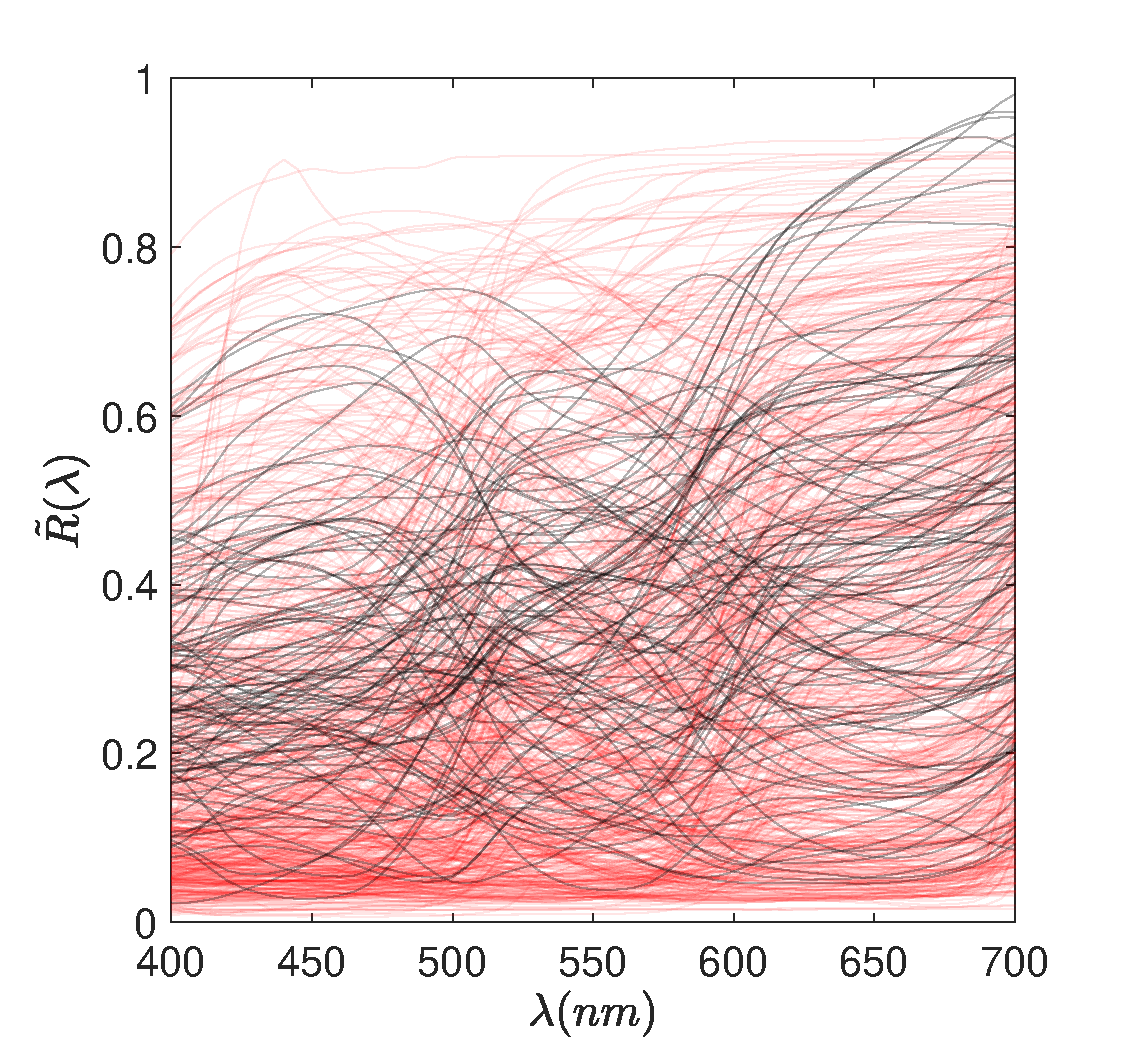
\includegraphics[width=\textwidth]{../Figures/Figure7/Figure7_a.pdf}
        \caption{Natural surface reflectance spectra}
        \label{fig:naturalSurface}
    \end{subfigure}
    \begin{subfigure}[b]{0.3\textwidth}
    \centering
        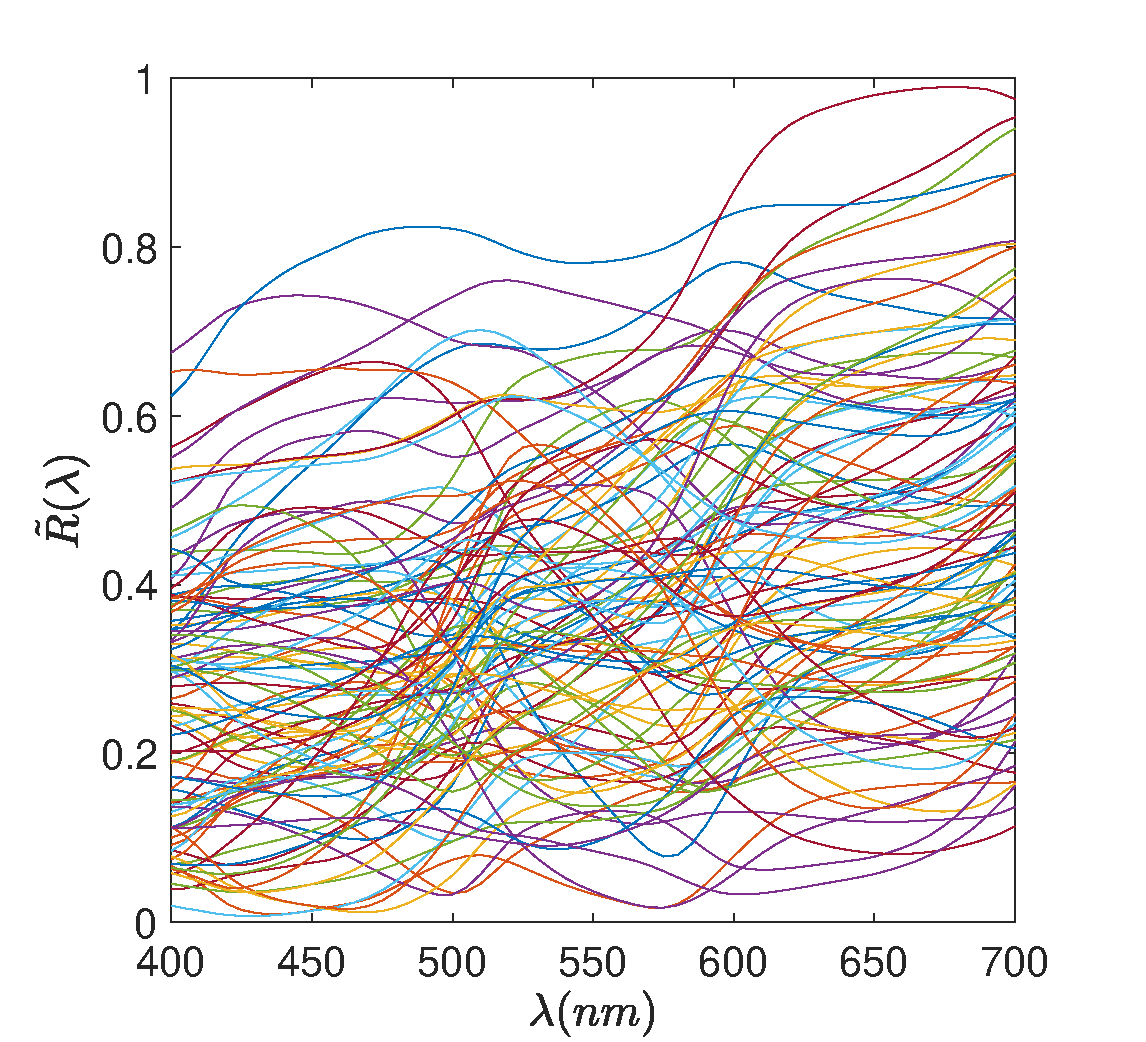
\includegraphics[width=\textwidth]{../Figures/Figure7/Figure7_b.pdf}
        \caption{Randomly generated samples}
        \label{fig:randomSurface}
    \end{subfigure}
    \begin{subfigure}[b]{0.3 \textwidth}
    \centering
        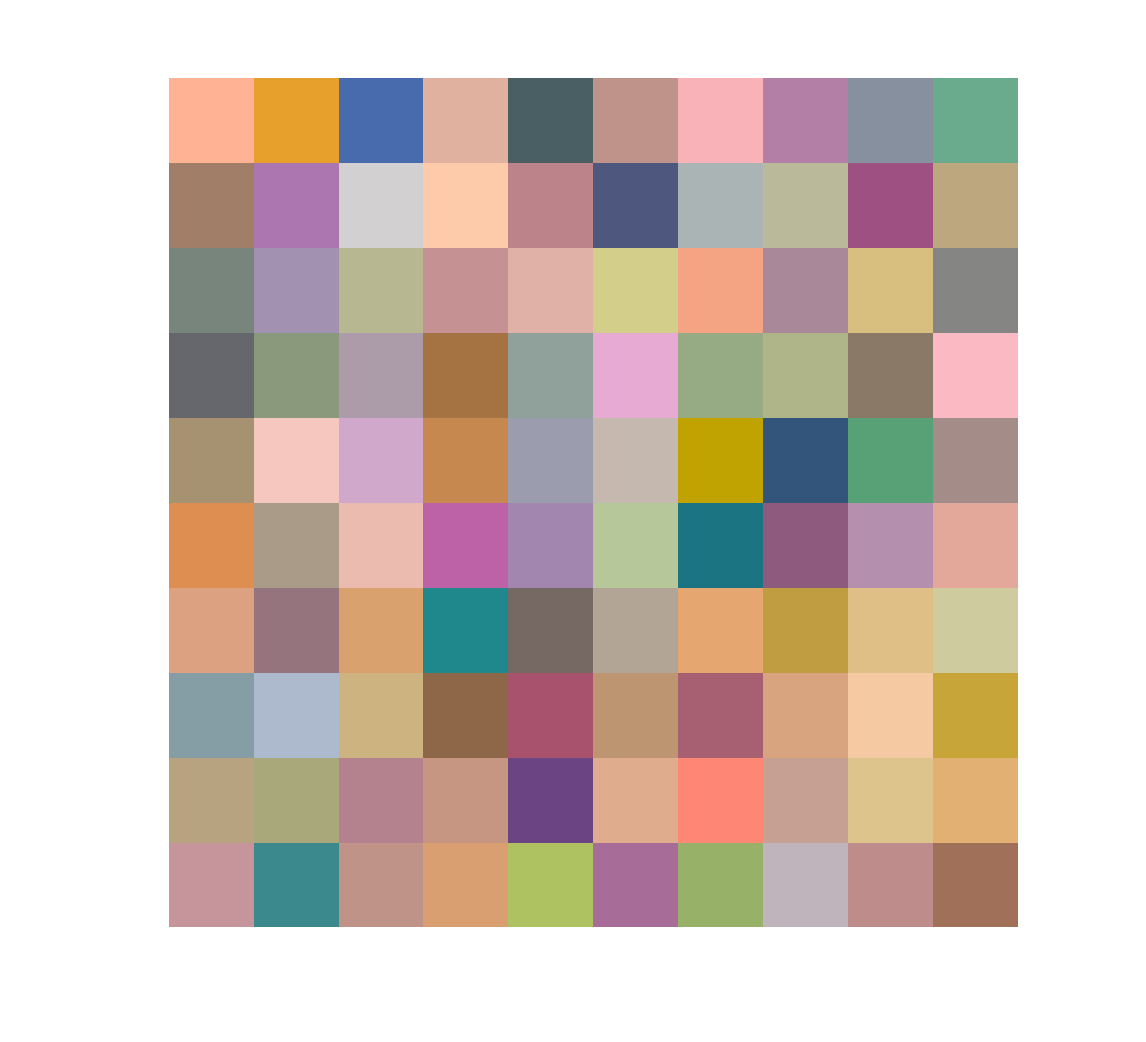
\includegraphics[width=\textwidth]{../Figures/Figure7/Figure7_c.pdf}
        \caption{sRGB rendition of samples from \ref{fig:randomSurface}}
        \label{fig:sRGBSurface}
    \end{subfigure}
    \caption{{\bf Generating random surface reflectance spectrum:} The surface reflectance spectra are generated by random sampling of natural surface reflectance spectra assuming a multivariate gaussian distribution. The mean and variance of the gaussian are chosen by projecting the natural dataset along PCA directions and taking the mean and covariance of the projections. (a) Natural surface reflectance spectra. (b) Randomly generated samples. (c) The sRGB renditions of the random samples generated in \ref{fig:randomSurface}.}\label{fig:surfaceReflectanceGeneration}
\end{figure}


The reflectance spectrum are generated similar to illumination spectrum. 
We have used the Munsell {(\it citation)} and vrhel {(\it citation)} surface reflectance 
datasets for sampling the reflectance. Let us denote the dataset of natural 
reflectance spectra as $R_i(\lambda)$, where $\{i \in [1,M]\}$ 
and $M$ is the total number of spectra in the dataset. To generate 
a random reflectance spectrum $\tilde{R}(\lambda)$, 
we first mean center the dataset by subtracting out the 
mean surface reflectance spectrum, $\bar{R}(\lambda)$,
from each surface reflectance spectrum.
$\bar{R}(\lambda)$ is obtained by taking the sample 
mean over all spectra in the dataset, i.e.,
$\bar{R}(\lambda) = \frac{1}{M} \sum_{i=1}^M R_i(\lambda)$. 
Thus we have the mean centered reflectance 
spectrum dataset as $R_i^{\rm MC}(\lambda) =  R_i(\lambda)-\bar{R}(\lambda)$. 
We decompose this as $R_i^{\rm MC}(\lambda) = \sum_j{w_{ij} \; {\bf \hat{e}}_j^{\rm PCA}}$. Here,
${\bf \hat{e}}_j^{\rm PCA}$s are PCA basis vectors obtained using SVD 
and $w_{ij}$s are the projections of $R_i^{\rm MC}(\lambda)$ along the PCA eigenvectors 
$\left( w_{ij} = R_i^{\rm MC}(\lambda)\cdot {\bf \hat{e}}_j^{\rm PCA}\right)$. The 
decomposition is approximated by summing over the PCA basis 
vectors corresponding to the largest six SVD eigenvalues. These six eigenvalues capture 
more than $92\%$ of the variance in the combined Munsell and vhrel datasets. To generate 
a new reflectance spectrum, a point is sampled randomly in this 
six dimensional sub-space using a multivariate normal 
distribution, with mean $\bar{w}_j = \frac{1}{M}\sum_i w_{ij}$, 
and co-variance $\Sigma_{jj'} = \frac{1}{M} \sum_i \left(w_{ij} -\bar{w}_j\right)\left(w_{ij'} -\bar{w}_{j'}\right) $. If the randomly sampled projection, $\tilde{w}_{ij}$, is 
such that $\left( 0 < \sum_j \tilde{w}_{ij}{\bf \hat{e}}_j^{\rm PCA} + \bar{R}(\lambda)<1\right) $ at every $\lambda$, the new surface reflectance 
is given as: $\tilde{R}_i(\lambda) =\sum_j \tilde{w}_{ij}{\bf \hat{e}}_j^{\rm PCA} + \bar{R}(\lambda)$.

% Figure 8
\begin{figure}
\centering
	\begin{subfigure}[b]{0.3 \textwidth}
    \centering
        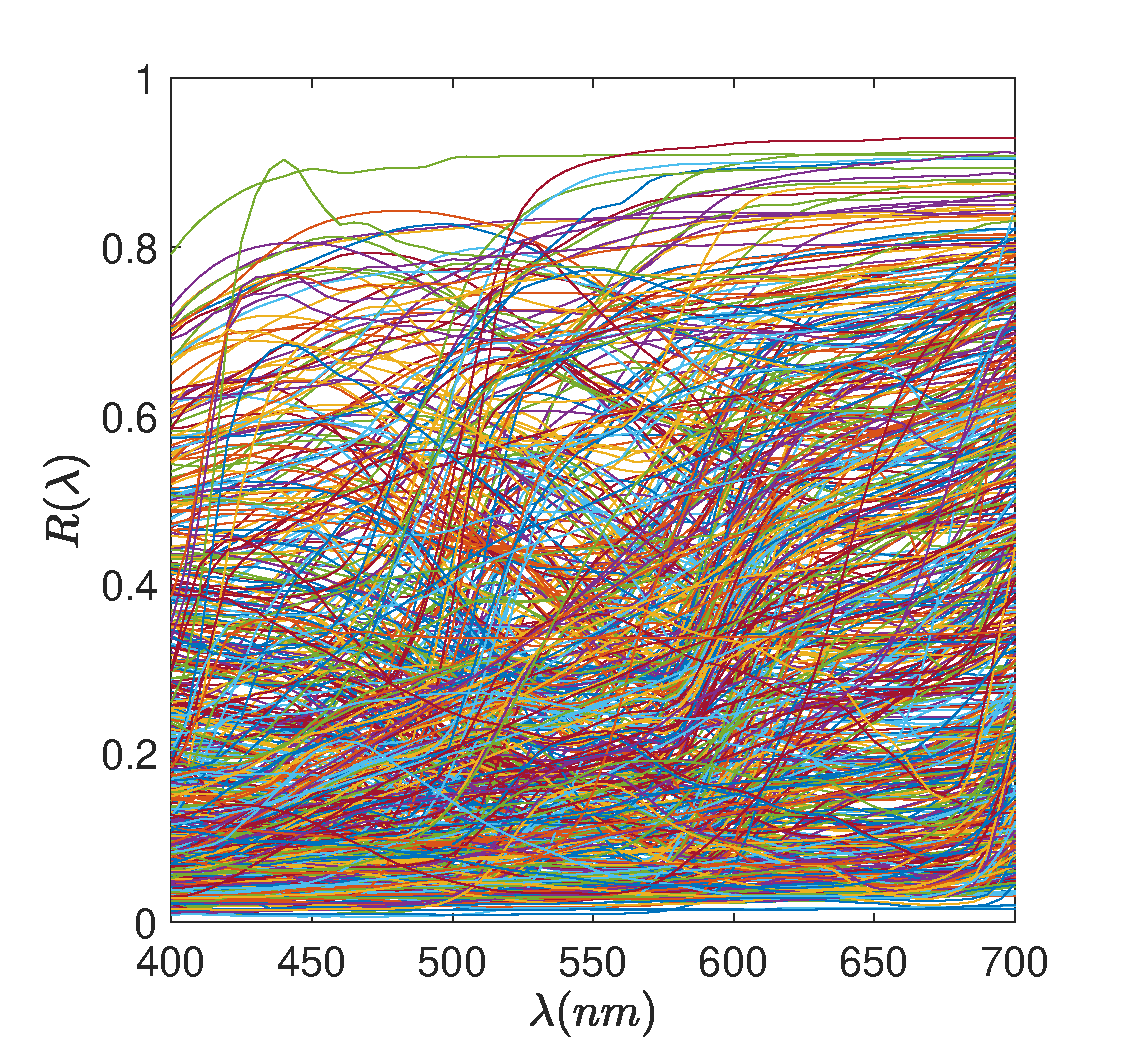
\includegraphics[width=\textwidth]{../Figures/Figure8/Figure8_a.pdf}
        \caption{Natural surface reflectance spectra}
        \label{fig:naturalSurfaceTarget}
    \end{subfigure}
    \begin{subfigure}[b]{0.3\textwidth}
    \centering
        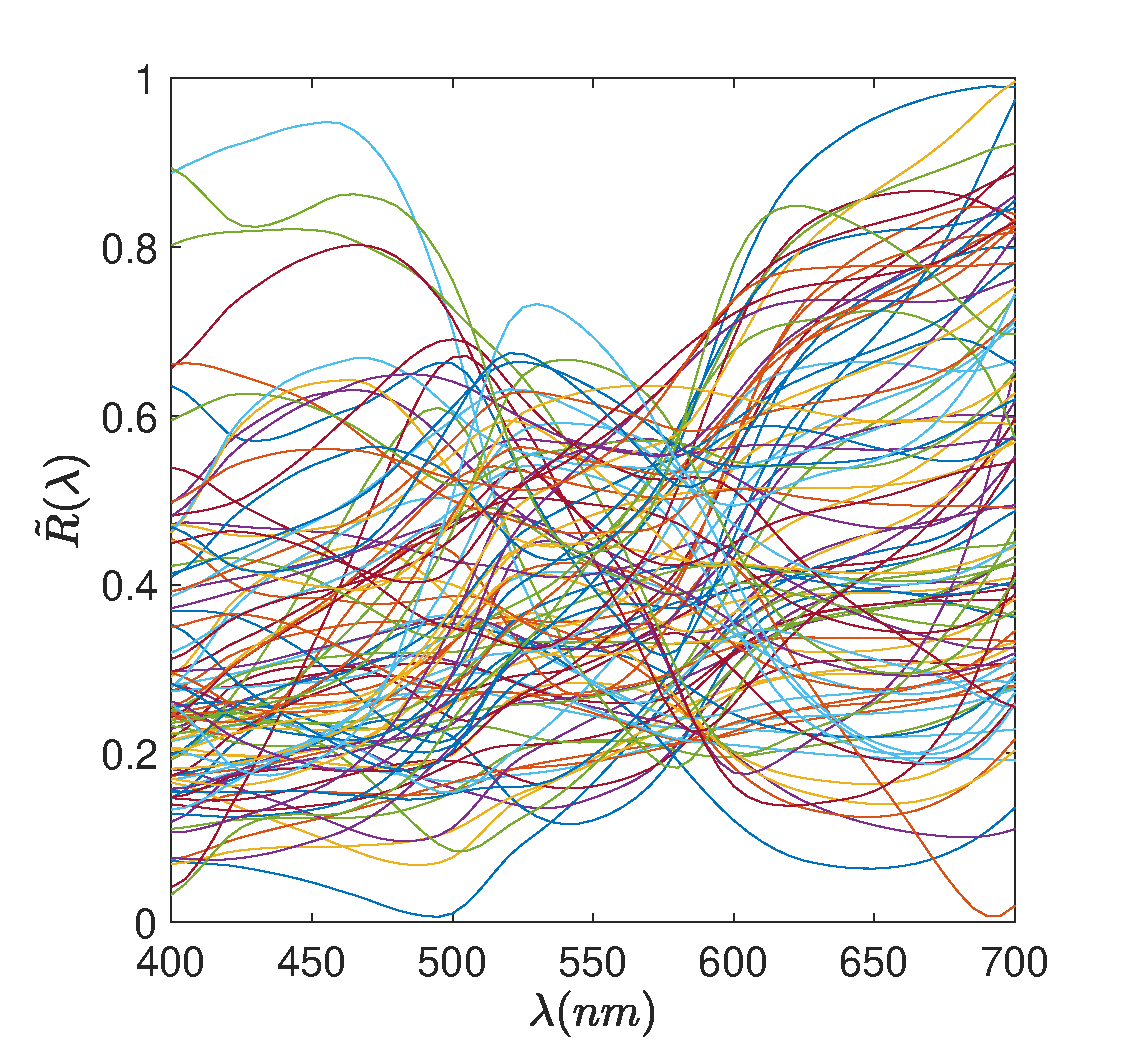
\includegraphics[width=\textwidth]{../Figures/Figure8/Figure8_b.pdf}
        \caption{Randomly generated target samples}
        \label{fig:randomSurfaceTarget}
    \end{subfigure}
    \begin{subfigure}[b]{0.3 \textwidth}
    \centering
        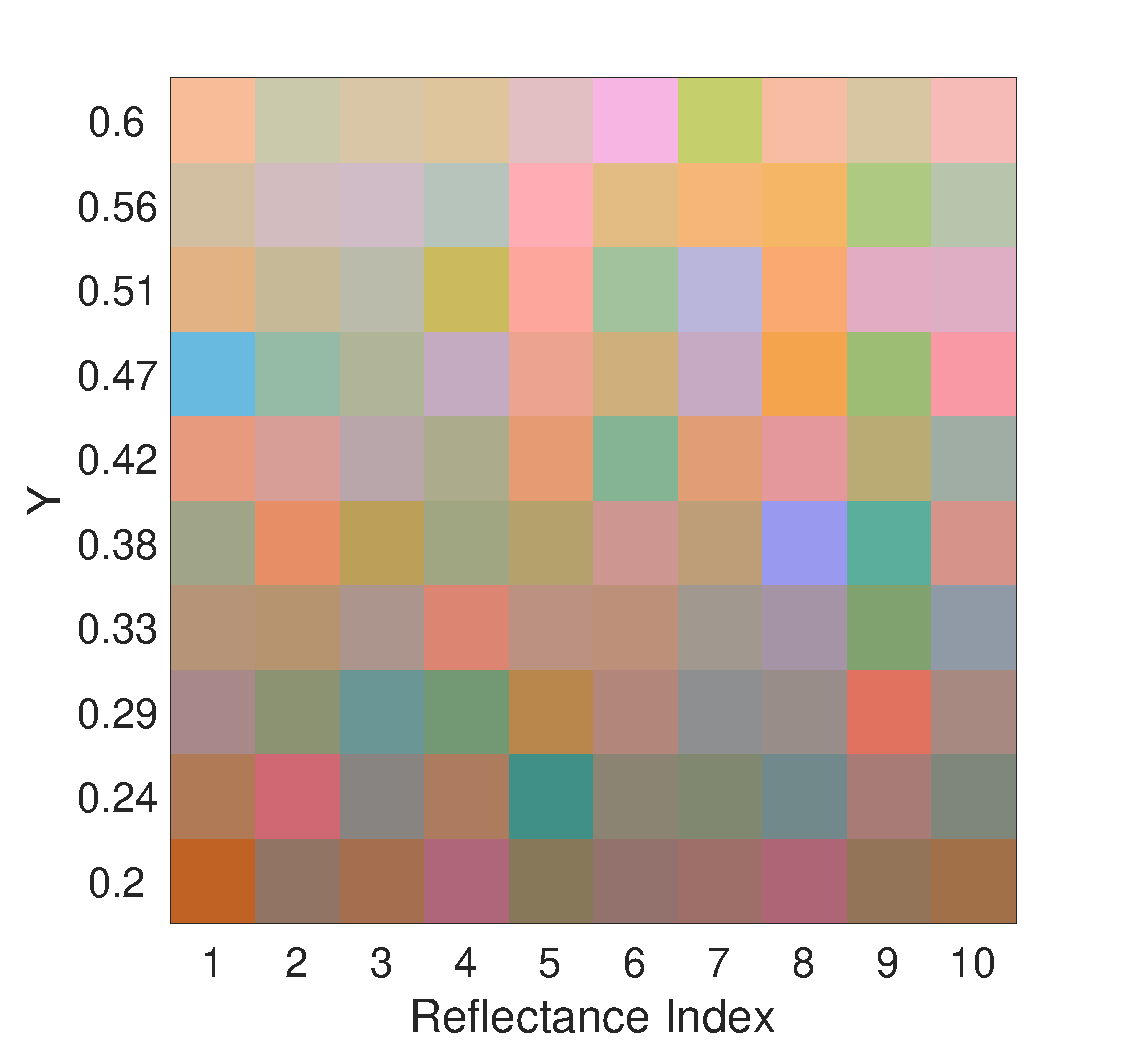
\includegraphics[width=\textwidth]{../Figures/Figure8/Figure8_c.pdf}
        \caption{sRGB rendition of samples from Fig.~\ref{fig:randomSurfaceTarget}}
        \label{fig:sRGBSurfaceTarget}
    \end{subfigure}
    \caption{{\bf Target object surface reflectance spectrum:} For getting the target object surface reflectance, we first generate the spectra similar to that of other objects and then rescale them appropriately to get the required perceived lightness. (a) Natural surface reflectance spectra. (b) Randomly generated samples for target reflectance. (c) The sRGB renditions of the random samples generated in Fig.~\ref{fig:randomSurfaceTarget}. We show 10 samples at 1 lightness levels.}\label{fig:targetSurfaceReflectance}
\end{figure}


For generating the target object reflectance at a particular lightness $(Y_{\rm T})$, the values in the spectrum are 
rescaled by a scalar such that the perceived lightness of the 
target surface under standard daylight illuminant $(D_{65}(\lambda))$ 
equals a designated value. The scaling equals $\frac{Y_{\rm T}}{\int d\lambda \tilde{R}(\lambda) D_{65}(\lambda) \bar{y}(\lambda)}$, with $\bar{y}(\lambda)$ being the CIE luminosity (or luminous efficiency) function. 
$\bar{y}(\lambda)$ describes the average spectral sensitivity of human visual 
perception of brightness. The target reflectance is given by: $\tilde{R}^{\rm T}_i(\lambda) =\tilde{R}_i(\lambda) \cdot\left(\frac{Y_{\rm T}}{\int d\lambda \tilde{R}(\lambda) D_{65}(\lambda) \bar{y}(\lambda)}\right)$.

% NEED TO DECIDE PRECISELY WHERE TO USE THIS PROSE AND  FIGURE
%Figure~\ref{sceneWithCroppedImage} illustrates the steps in this process for one scene.  We start with how we generate a single labeled set of cone responses
%We call our image generation software Virtual world color constancy (VWCC). The details of the software are provided in the supplementary information section. To generate an image, we first select a 3D scene, a target object and a light source from the set of predefined scenes and objects in VWCC. The target object and the light source are inserted in the 3D scene. Fig.\ref{fig:3DScene} shows a 2D sRGB rendition of the 3D scene used in our analysis. The green sphere in the middle is the target object. The light source is not in the camera field of view. Next, we assign a surface reflectance spectrum and an illumination spectrum to each object and light source in the scene. For the target object the surface reflectance is assigned such that the perceived lightness of the target object under D65 daylight spectrum has a fixed value. Now we render a $320\times 240$ pixel$^2$ 2d multispectral images of the scene at 31 frequencies (equal linear spacing between 400 nm - 700 nm) using a graphics rendering system called Mitsuba \cite{jakob2015mitsuba}. For each of the three case, we generate hundreds of such scenes and corresponding multispectral images at 10 linearly spaced lightness levels between 0.2 and 0.6 (see below). We crop a 51x51 pixel$^2$ part of the multispectral image containing the target object for further analysis (\ref{fig:croppedImage}). Fig. \ref{fig:studiedCases} shows examples of such cropped image at 3 lightness levels for the three cases considered in this work.

% Figure 9: Methods
\begin{figure}
\centering
\begin{subfigure}[b]{0.25 \textwidth}
		\centering
        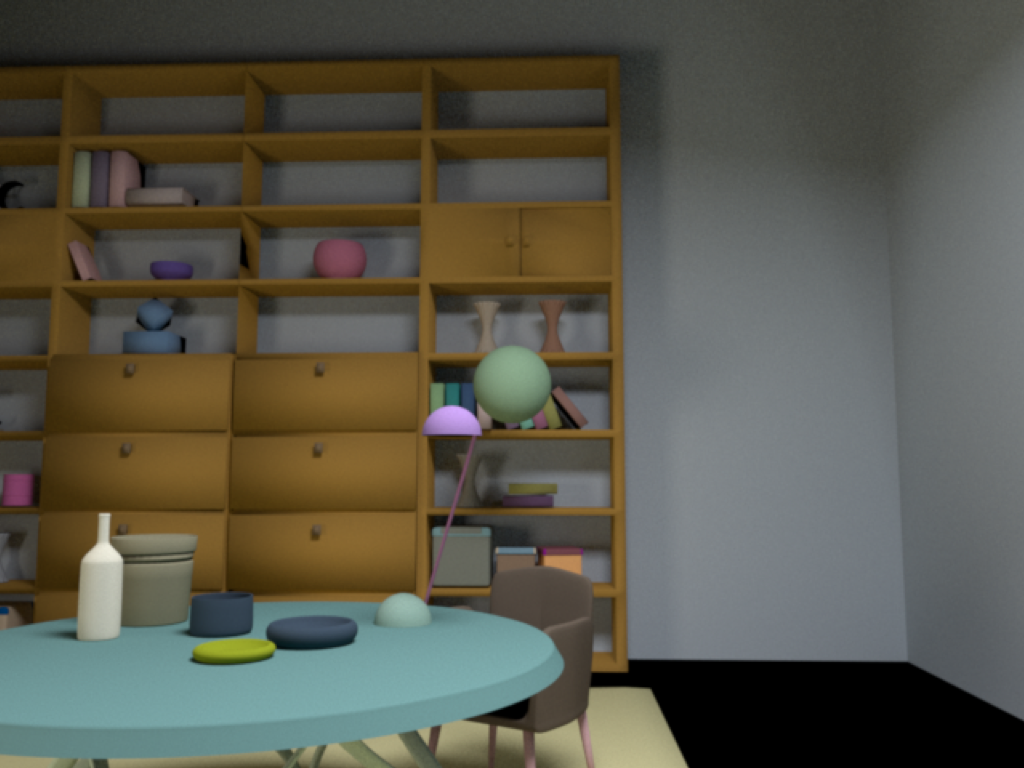
\includegraphics[width=\textwidth]{../Figures/Figure9/Figure9_a.png}
        \caption{A typical 3D Scene}
        \label{fig:3DScene}
    \end{subfigure}
    ~ %add desired spacing between images, e. g. ~, \quad, \qquad, \hfill etc. 
      %(or a blank line to force the subfigure onto a new line)
    \begin{subfigure}[b]{0.19 \textwidth}   
    \hspace{0.1 \textwidth}
        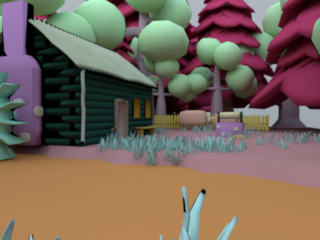
\includegraphics[width=\textwidth]{../Figures/Figure9/Figure9_b.png}
        \caption{Cropped Image}
        \label{fig:croppedImage}
    \end{subfigure}
    ~ %add desired spacing between images, e. g. ~, \quad, \qquad, \hfill etc. 
    %(or a blank line to force the subfigure onto a new line)
    \begin{subfigure}[b]{0.19 \textwidth}
    \hspace{0.1 \textwidth}
        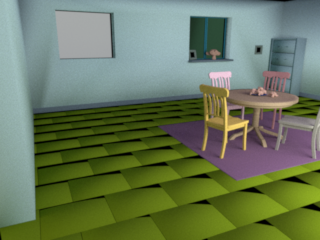
\includegraphics[width=\textwidth]{../Figures/Figure9/Figure9_c.png}
        \caption{Optical Image}
        \label{fig:croppedImageWithMosaic}
    \end{subfigure}
    ~
    \begin{subfigure}[b]{0.2 \textwidth}
        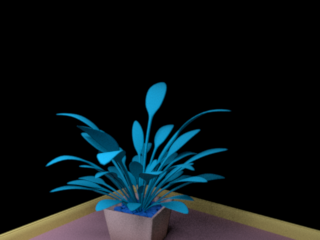
\includegraphics[width=\textwidth]{../Figures/Figure9/Figure9_d.png}
        \caption{LMS cone contrast}
        \label{fig:coneContrast}
    \end{subfigure}
    \label{fig:sceneWithCroppedImage}
    \caption{{\bf Generating labeled dataset for computational analysis:}  For the supervised approach employed in this work, the labeled database is generated as follows: (a) A 3D virtual scene, a target object and a light source is selected from the VWCC library. The target object is placed in the camera field of view and assigned a reflectance spectrum with a specific lightness. After assigning spectra to other objects and lights sources in the scene, a multispectral image of the scene is rendered using Mitsuba graphics rendering software. (b) A part of the image, containing the target object, is cropped from the image. (c) The response of the retinal cones to the cropped image is simulated using a model of the visual system. Fig.\ref{fig:croppedImageWithMosaic} shows the optical image incident on the cone mosaic and the location and the identity of the cones (L cones: Red, M cones: Green, S cones: Blue). See text for the details of the model. (d) The cone response are interpolated to get the response of all the three types at each location (demosaicing). Finally, the demosaic response is contrast normalized (see text).}
\end{figure}

\subsection{Model of Visual System} \label{method:Isetbio}

Finally, these multispectral images are used to simulate retinal cone responses using \href{https://github.com/isetbio}{Isetbio} software.

To generate the retinal response one needs to specify the retinal cone mosaic and the size of the retinal image. The retinal cone mosaic is specified in terms of the total number of cones and the proportion of the long(L), medium(M) and the short(S) cones in the mosaic. With these parameters, the software generates the specified number of LMS cones with random positions on a square grid. The size of the retinal image is specified in terms of the field of view and object distance from the eye. 


We simulate visual system response using \href{http://isetbio.org}{Isetbio} software toolbox. Isetbio simulates a model of the visual system accounting for cornea, pupil size, lens and physiological optics. We use the multispectral cropped image (Fig.~\ref{fig:croppedImage}) as the optical stimulus to simulate the response of the cones in the retina. The cropped image patch is assumed to cover a $1^{\circ}$ field of view at a distance of 1 m. The retinal cone mosaic is modeled as a square grid with 51x51 cones in the l:m:s ratio 0.6:0.3:0.1. The response of the cones are measured as the number of isomerizations in the cone segment ({\it over what time ??}). The cone response functions are normalized by the total area under the response curves to model the amplification of the S cone response downstream and thus have comparable number if isomerizations in L, M and S cones. Further, to get the response of each cone class at each position on the retinal mosaic, we interpolate the response of each cone class. Thus we get a $51 \times 51$ cone response image for each cone class.

The three $51 \times 51$ cone response matrix corresponding to L, M and S cones are then reshaped into a $7803 \times 1$ vector. To model the contrast adaptation in the visual system, we perform a contrast normalization of the vector by subtracting and dividing by the mean. We further  rescale the vector to have norm 1. The cone-response vectors corresponding to the N images for each case are concatenated into a column-wise contrast normalized matrix $C_{7803\times N}$. The corresponding labels are represented by the row vector $Y_{1\times N}$.

\subsection{Supervised Learning methods} \label{method:SupervisedLearning}
\subsubsection*{Linear Regression} For linear regression, we solve the equation $A_{(1,3)}*C_{(3,N)} = Y_{(1,N)}$ for the regression parameters $A_{(1,3)}$. Here, $C_{(3,N)}$ has the contrast normalized matrix of LMS cone responses of the center pixel. Each column corresponds to the N images in the dataset. The rows correspond to the contrast normalized L, M and S cones response of the center pixel for each image. The L, M and S response to the center pixel on the target object is calculated by taking the average of a 3x3 patch of cones near the center of the target.The (unknown) regression parameters $A$ are obtained using Matlab linear regression function. 

\subsubsection*{SVD regression}
SVD regression is a generalization of principal component analysis for labeled data \cite{ranganNotes}. Briefly, given an image dataset matrix $C_{M \times N}$ and labels $Y_{1\times N}$, the method finds unit vectors such that the projection of the data along this vector maximizes the separation of the images with different labels, while clustering the images with similar labels together. Mathematically, the method searches for a direction $\hat{u}$ such that minimize the cost function:
\begin{align}
S = \sum\limits_{j,j'}\left(\hat{u}^\intercal C(:,j) - \hat{u}^\intercal C(:,j')\right)^2 \left(Y(j)-Y(j') \right)^2,
\end{align} 
where $C(:,j)$ represents the $j$'th column/image of the data matrix $C$. The direction of minimum cost is given by the eigenvector corresponding to the largest eigenvalue of the matrix:
\begin{align}
N C Y_D^2 C^\intercal - 2(Y*\mathbbm{1})C Y_D C^\intercal + (Y*Y^\intercal) (CC^\intercal)-C Y_{D}^2\mathbbm{1}\mathbbm{1}^\intercal C^\intercal +2 C Y_{D} \mathbbm{1}\mathbbm{1}^\intercal Y_{D} C^\intercal - C \mathbbm{1}\mathbbm{1}^\intercal Y_{D}^2 C^\intercal.
\end{align}
Here, $Y_{D}$ is a diagonal matrix with the elements of the labels vector $Y$ along the diagonal, and $\mathbbm{1}$ is a $N\times 1$ vector of ones.

\subsubsection*{Accuracy maximization analysis}
 \cite{geisler2009optimal,burge2017accuracy} is a Bayesian ideal observer model for task specific dimensionality reduction. Given a labeled training set, a noisy response model, and a cost function, AMA returns a set of linear receptive fields that are optimal for performing a task. The task is implicitly defined in terms of the labels. The optimal filters are the ones whose noisy response to the stimuli, as given by the specified response model, minimizes the cost function over the training set. 

Let us assume that the labels ($Y$) take one of the $N_{\nu}$ possible values $\{Y_k: k\in[1,N_{\nu}] \}$ and the $l$'th stimuli corresponding to the $k$'th category of the labels is represented as $s_{kl}$. Let us assume that there is a set of linear filters {\textbf{\textit f}} which when acting on $s_{kl}$ gives the response ${\textbf{\textit R}}_{kl}$. Let's say we have a decoder $g$ that takes ${\textbf{\textit R}}_{kl}$ as the input and returns an estimate of the latent variable ($Y_k$) corresponding to the stimuli $s_{kl}$ as $\hat{Y}_{kl}$. Given this estimate, one can define a cost function $\mathcal{C}_{kl}(Y_{kl},\hat{Y}_{kl})$ corresponding to specific response ${\textbf{\textit R}}_{kl}$ and a mean cost $\bar{\mathcal{C}}_{kl}(Y_{kl},\hat{Y}_{kl})$ corresponding to the average response $r_{kl} = \langle{\textbf{\textit R}}_{kl}\rangle$. 

Accuracy maximization analysis (AMA) finds the set of optimal filters ${\textbf{\textit f}}^{\rm opt}$ that minimize the average cost function over the entire dataset $\{s_{kl}: k\in[1,N_{\nu}], l\in[1,N_k]\}$. $N_{\nu}$ is the total number of labels and $N_{k}$ is the number of stimuli corresponding to the label $Y_k$. Thus,
\begin{align}
{\textbf {\textit f} }^{\rm opt} = \argmin_{\textbf {\textit f} } \sum_{kl} \bar{\mathcal{C}}_{kl}.
\label{eq:fopt}
\end{align}

AMA employs the Bayes optimal decoder ($g$) to estimate the optimal estimate. The Bayesian decoder computes the posterior probability of the latent variable $p(X|{\textbf {\textit R}})$ and reads out the optimal estimate $\hat{Y}^{\rm opt}$ from the posterior as the value that minimizes the cost. By Bayes' theorem, the posterior probability can be written as:
\begin{align}
p(Y_k|{\textbf {\textit R} }_{kl}) = \frac{p({\textbf {\textit R} }_{kl}|Y_k)p(Y_k)}{\sum\limits_{i=1}^{N_{\nu}}{p({\textbf {\textit R} }_{kl}|Y_i)p(Y_i)}}.
\label{eq:posterior}
\end{align}
As the conditional probability of the filter response is:
\begin{align}
p({\textbf {\textit R} }_{kl}|Y_k) = \sum\limits_{m=1}^{N_k}p({\textbf {\textit R} }_{kl}|{\textbf {\textit s} }_{km})p({\textbf {\textit s} }_{km}|Y_k),
\label{eq:condProb}
\end{align}
using Eq.~\ref{eq:condProb} in Eq.~\ref{eq:posterior} we get:
\begin{align}
p(Y_k|{\textbf {\textit R} }_{kl}) = \frac{\left[\sum\limits_{m=1}^{N_k}p({\textbf {\textit R} }_{kl}|{\textbf {\textit s} }_{km})p({\textbf {\textit s} }_{km}|Y_k)\right]p(Y_k)}{\sum\limits_{i=1}^{N_{\nu}}{\left[\sum\limits_{j=1}^{N_j}p({\textbf {\textit R} }_{il}|{\textbf {\textit s} }_{ij})p({\textbf {\textit s} }_{kj}|Y_i)\right]p(Y_i)}}
\label{eq:finalPosterior}
\end{align}
Since, $p({\textbf {\textit s} }_{km}|Y_k) = \frac{1}{N_k}$, and $p(Y_k)=\frac{N_k}{N}$, where $N = \sum\limits_{k=1}^{N_{\nu}}N_{k}$ is total number of samples in the training set, Eq.\ref{eq:finalPosterior} simplifies to
\begin{align}
p(Y_k|{\textbf {\textit R} }_{kl}) = \frac{\left[\sum\limits_{m=1}^{N_k}p({\textbf {\textit R} }_{kl}|{\textbf {\textit s} }_{km}) \frac{1}{N_k}\right]\frac{N_k}{N}}{\sum\limits_{i=1}^{N_{\nu}}{\left[\sum\limits_{j=1}^{N_j}p({\textbf {\textit R} }_{il}|{\textbf {\textit s} }_{ij}) \frac{1}{N_i}\right]\frac{N_i}{N}}} = \frac{\sum\limits_{m=1}^{N_k}p({\textbf {\textit R} }_{kl}|{\textbf {\textit s} }_{km})}{\sum\limits_{i=1}^{N_{\nu}}{\sum\limits_{j=1}^{N_j}p({\textbf {\textit R} }_{il}|{\textbf {\textit s} }_{ij})}}.
\label{eq:simplifiedPosterior}
\end{align}
Now if the cost associated with the latent variable $Y_k$ and the estimate $\hat{Y}_k$ is $\gamma (Y_k,\hat{Y}_k)$, we have  
\begin{align}
\mathcal{C}_{kl} = \sum\limits_{u=1}^{N_{\nu}}\gamma(X_u,\hat{Y}_u)p(X_u|{\textbf{\textit R}}_{kl}),
\end{align}
and the mean cost associated with the training set is $\bar{\mathcal{C}} = \frac{1}{N} \sum\limits_{k,l}\bar{\mathcal{C}}_{kl} = \frac{1}{N} \sum\limits_{k,l}\langle \mathcal{C}_{kl}\rangle_{{\textbf{\textit R}}_{kl}}$. The optimal AMA filters are obtained by minimizing $\bar{\mathcal{C}}$ over the filter set ${\textbf {\textit f} }$ (Eq.\ref{eq:fopt}). The filters are obtained using gradient descent.

In this work, we assume the noisy response model to be a multivariate gaussian. For a stimuli $s_{kl}$, the noisy response vector ${\textbf{\textit R}}_{kl} = \left[{\textbf{\textit R}}_{kl,1},{\textbf{\textit R}}_{kl,2},\dots,{\textbf{\textit R}}_{kl,q}\right]$ to the set of filters ${\textbf{\textit f}} = \left[{\textbf{\textit f}}_{kl,1},{\textbf{\textit f}}_{2},\dots,{\textbf{\textit f}}_{q}\right]$ is given by $\mathcal{N}({\textbf{\textit r}}_{kl}, \Sigma)$, with mean response vector ${\textbf{\textit r}}_{kl} = \left[{\textbf{\textit r}}_{kl,1},{\textbf{\textit r}}_{kl,2},\dots,{\textbf{\textit r}}_{kl,q}\right] = \left[{\textbf{\textit f}}_{1}\cdot s_{kl},{\textbf{\textit f}}_{2}\cdot s_{kl}\dots,{\textbf{\textit f}}_{q}\cdot s_{kl}\right]$ and the covariance matrix as the diagonal matrix $\Sigma$ with variances $\left(\sigma_1^2, \sigma_2^2,\dots, \sigma_q^2 \right)$. We assume $\sigma_i^2 = \alpha |r_i| + \sigma_0^2$, $|{\textbf{\textit f}}_{kl,i}|=1$ and $s_{kl}$ to be zero mean contrast normalized, i.e., $\langle{s_{kl}}\rangle = 0$ \& ${|s_{kl}|=1}$.

\section{Results} \label{Results}
\subsection{Optimal receptive fields show a center surround structure}
Fig.~(\ref{fig:case9AllResults}-\ref{fig:case12AllResults}) shows the RFs, the linear response of these RFs training dataset and the lightness estimates of the test data for the three cases described above. We show the first two RFs for SVD and AMA methods (Fig.~(\ref{fig:case9AllResults}-\ref{fig:case12AllResults})(a-b)). The RFs are ranked in ascending order of the value of the cost function. Thus the first RF corresponds to the direction along which the projection of the data gives the minimum cost. The L, M and S components give the weights for the linear sum of the cone responses for the three cone types. The salient features are the center surround structure of the RFs and the higher weights of the L and M cones, compared to the S cones. 

For case 1, since the illuminant and the background are fixed, all the information is in the central target object reflectance. Thus, the RFs weights are mostly concentrated around the center. For case 2, while the target and the illuminant spectra varies, the background object spectra is fixed. Hence, the lightness can be estimated by simply from the contrast between the response of the cones corresponding to the target and the background. Thus, while the RFs show a trend of weights concentrated at the center similar to case 1, there is large negative contribution from the surround. The spatial features of the RFs are due the stereotypical geometry of the images (see SI). For case 3, has a similar center surround structure with more prominent features of the background as we also vary the spectra of the background objects. Again, the spatial features are a result of the stereotypical geometry of the images.

%% Figure 10
\begin{figure}
\centering
\begin{subfigure}[b]{0.27 \textwidth}
		\centering
        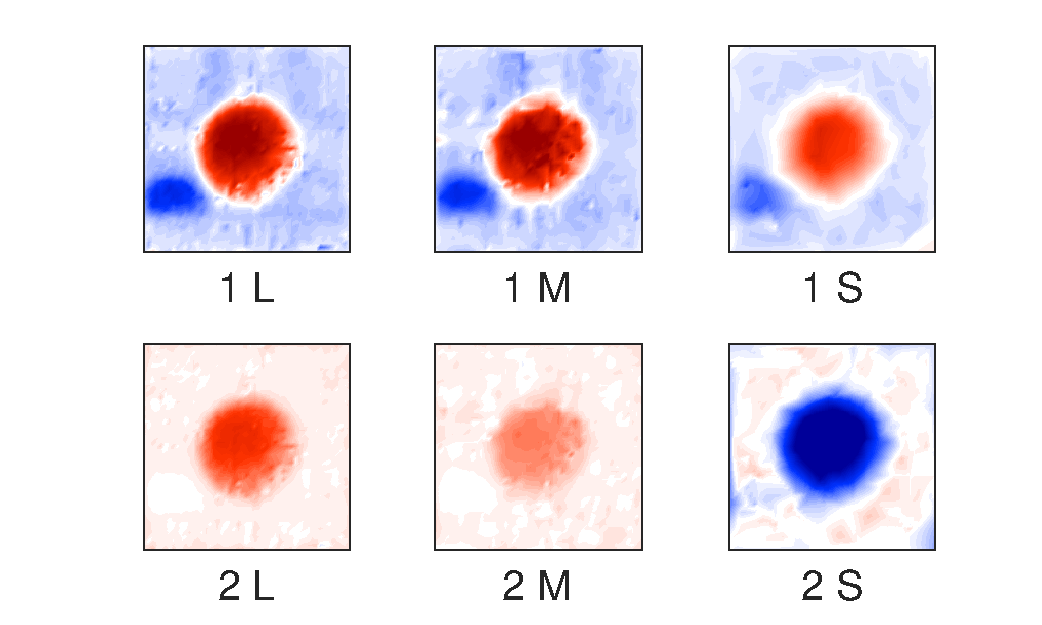
\includegraphics[width=\textwidth]{../Figures/Figure10/Figure10_a.pdf}
        \caption{SVD First 2 RFs}
        \label{fig:case9SVD}
    \end{subfigure}
    \begin{subfigure}[b]{0.27 \textwidth}   
        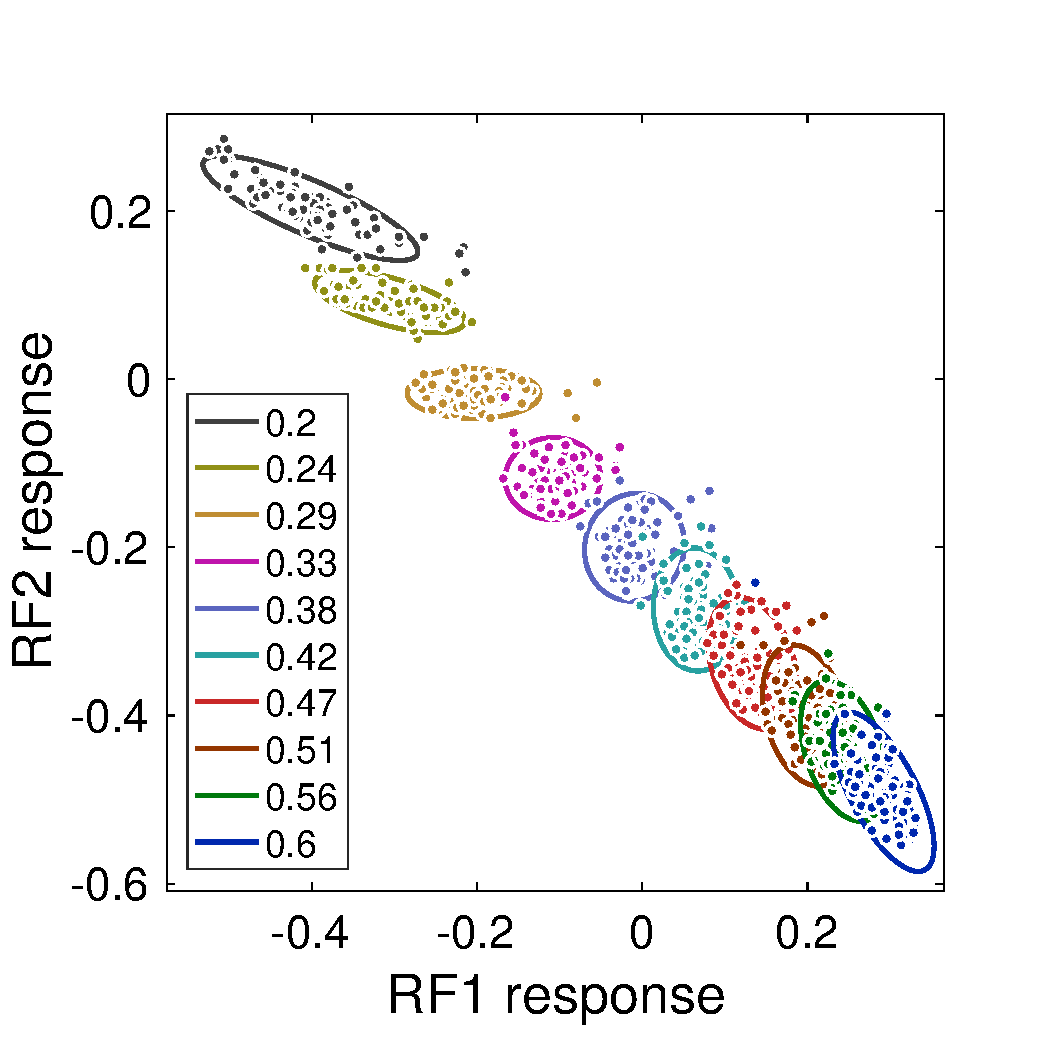
\includegraphics[width=\textwidth]{../Figures/Figure10/Figure10_b.pdf}
        \caption{AMA First 2 RFs}
        \label{fig:case9AMA}
    \end{subfigure}
        \begin{subfigure}[b]{0.20 \textwidth}
        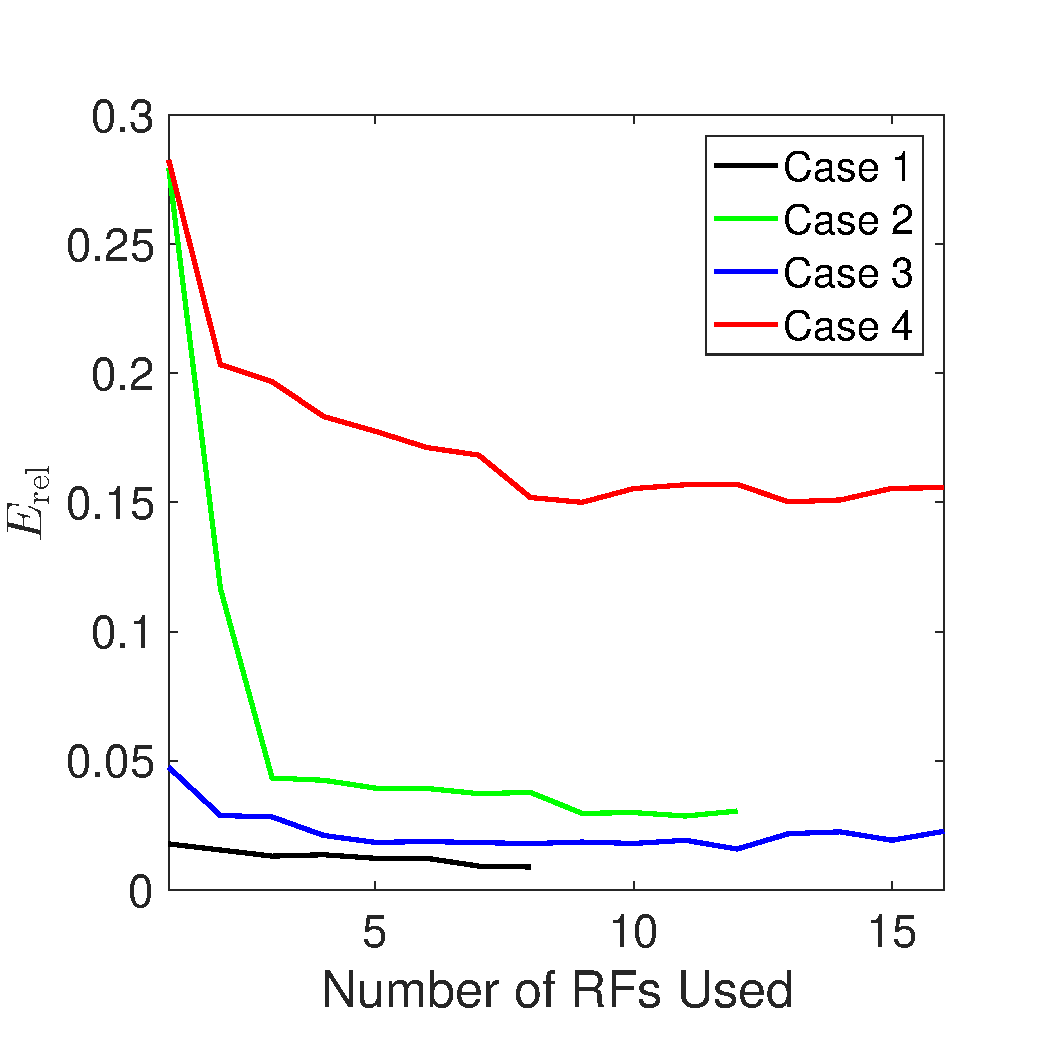
\includegraphics[width=\textwidth]{../Figures/Figure10/Figure10_c.pdf}
        \caption{AMA RF Response}
        \label{fig:case9FiltersResponse}
    \end{subfigure}
        \begin{subfigure}[b]{0.20 \textwidth}
        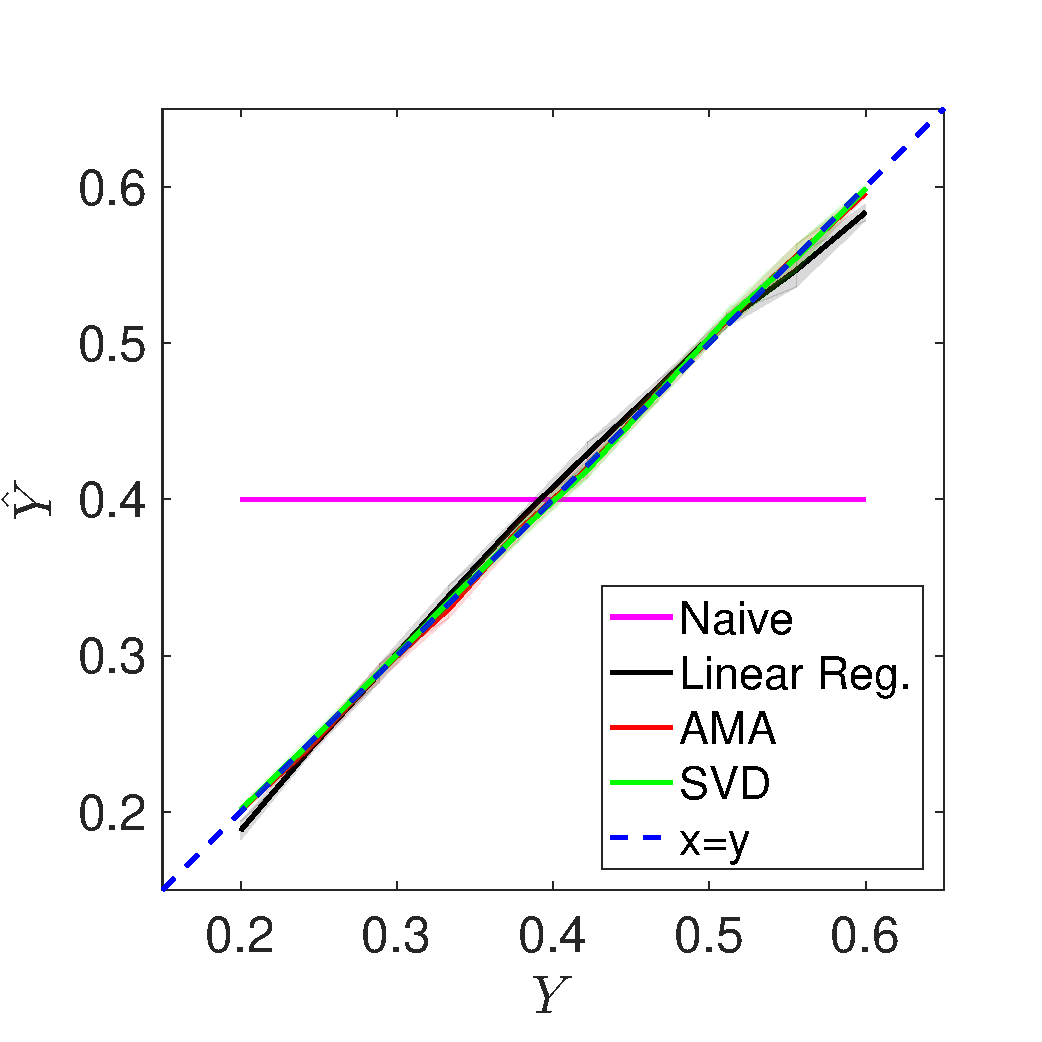
\includegraphics[width=\textwidth]{../Figures/Figure10/Figure10_d.pdf}
        \caption{Lightness Estimates}
        \label{fig:case9Results}
    \end{subfigure}    
    \caption{{\bf Receptive fields and lightness estimates. Case 1:} (a) First two receptive fields produced by the SVD method. Along the row we show the filters corresponding to the L cones, M cones and Scones (left to right). (c) First two receptive fields produced by the SVD method. (c) The response of the stimuli to the first two AMA filters. The responses are grouped with the label of the stimuli. As is clear, the response separate out quite well in this case, making the estimation easy (d) The estimates of the target object standard lightness. The naive method produces the mean value of the target luminance used in the analysis. The shaded region corresponds to 1 sigma standard deviation.}
\label{fig:case9AllResults}
\end{figure}

%% Figure 11
\begin{figure}
\centering
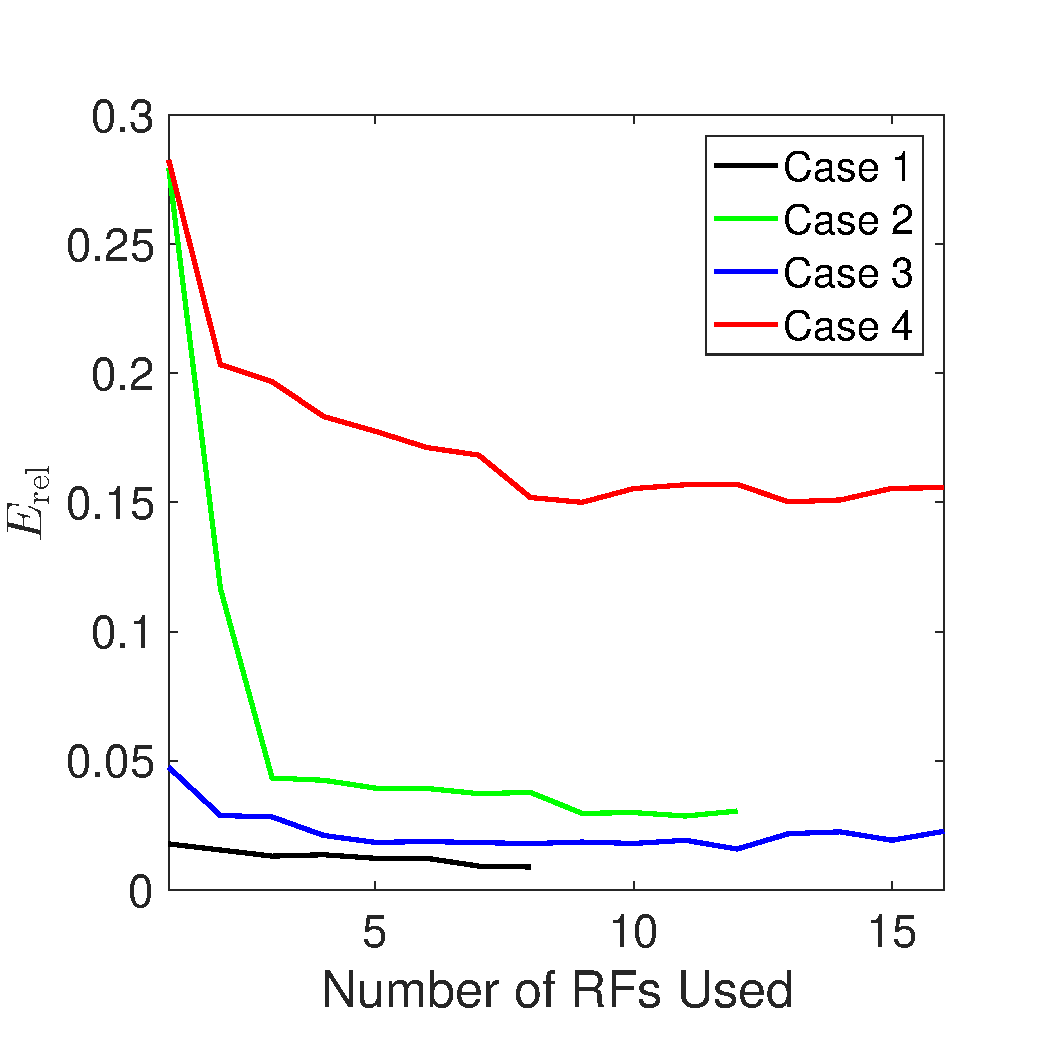
\includegraphics[width=0.3\textwidth]{../Figures/Figure11/Figure11.pdf}
\caption{{\bf Performance with number of RFs used for estimation:} Most of the information is captured by the first two filters. We have used the first 8 RFs for estimating the lightness.}
\label{fig:RMSEvsNFilters}
\end{figure}




% Figure 12
\begin{figure}
\centering
\begin{subfigure}[b]{0.27 \textwidth}
		\centering
        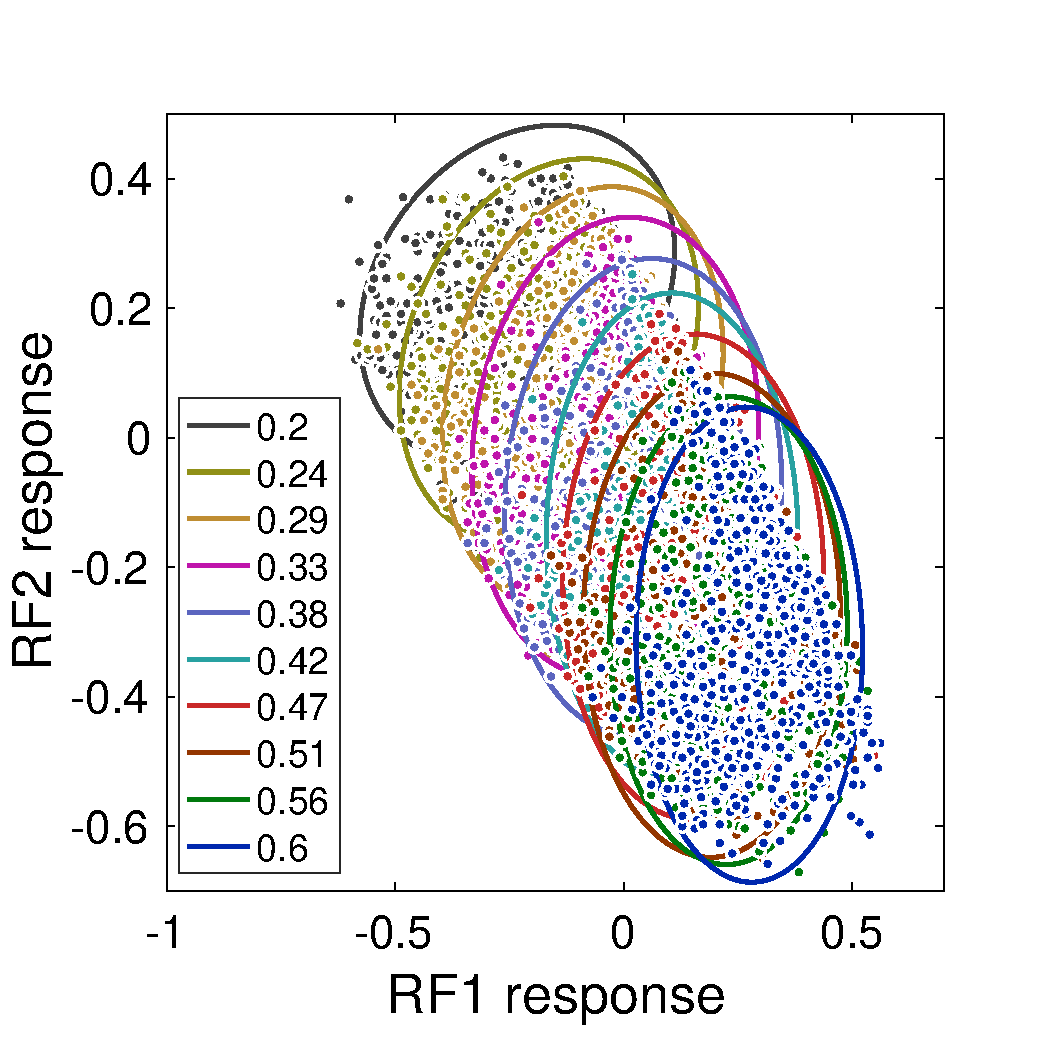
\includegraphics[width=\textwidth]{../Figures/Figure12/Figure12_a.pdf}
        \caption{SVD First 2 RFs}
        \label{fig:case10SVD}
    \end{subfigure}
    \begin{subfigure}[b]{0.27 \textwidth}   
        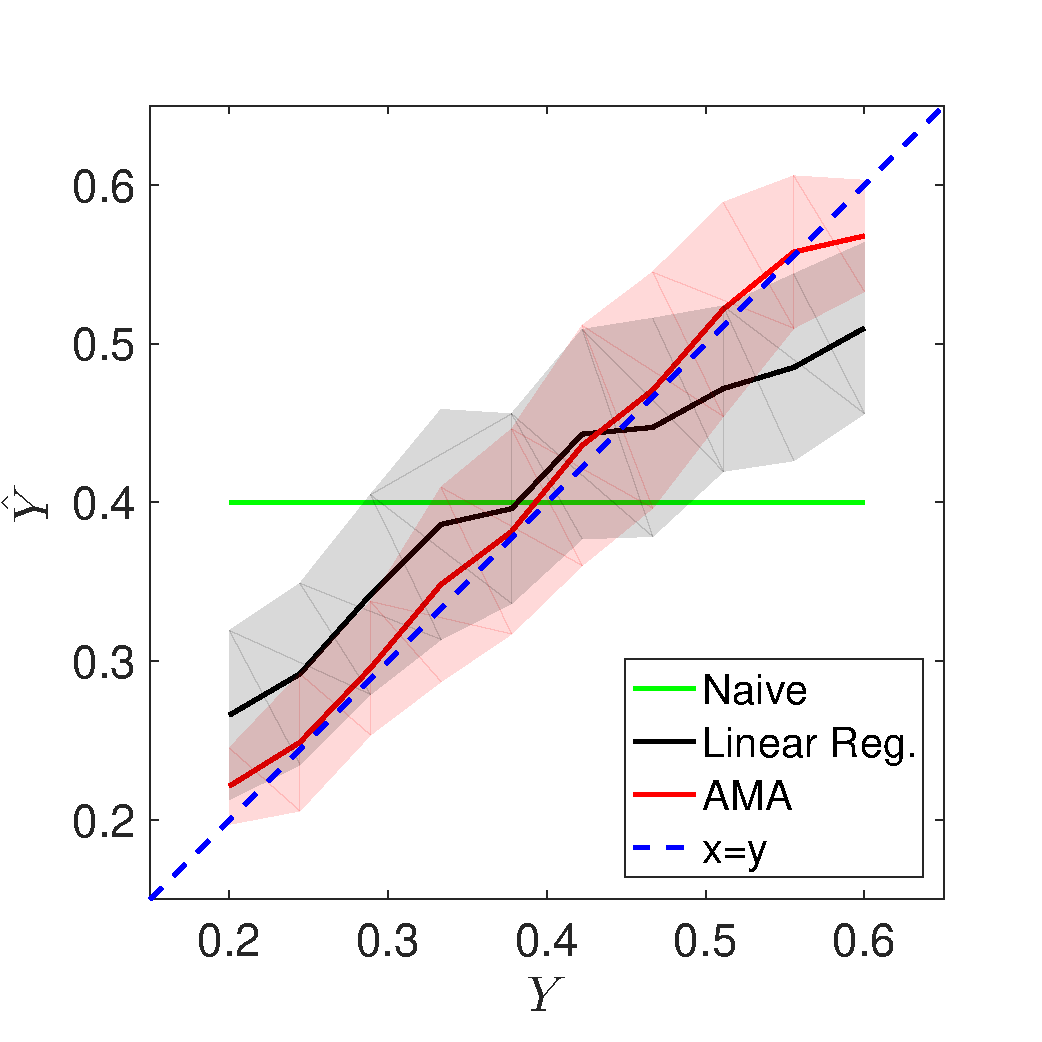
\includegraphics[width=\textwidth]{../Figures/Figure12/Figure12_b.pdf}
        \caption{AMA First 2 RFs}
        \label{fig:case10AMA}
    \end{subfigure}
        \begin{subfigure}[b]{0.20 \textwidth}
        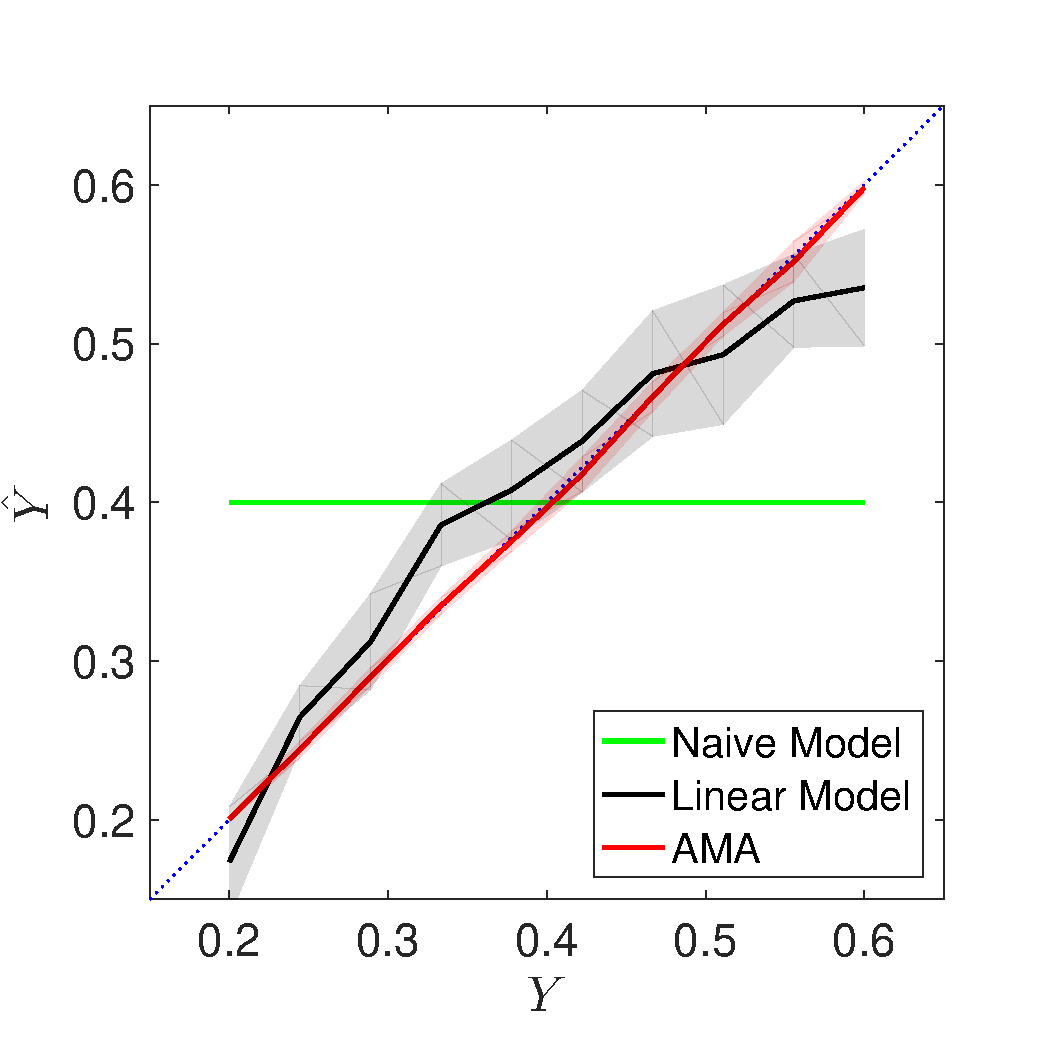
\includegraphics[width=\textwidth]{../Figures/Figure12/Figure12_c.pdf}
        \caption{AMA RF Response}
        \label{fig:case10FiltersResponse}
    \end{subfigure}    
        \begin{subfigure}[b]{0.2 \textwidth}
        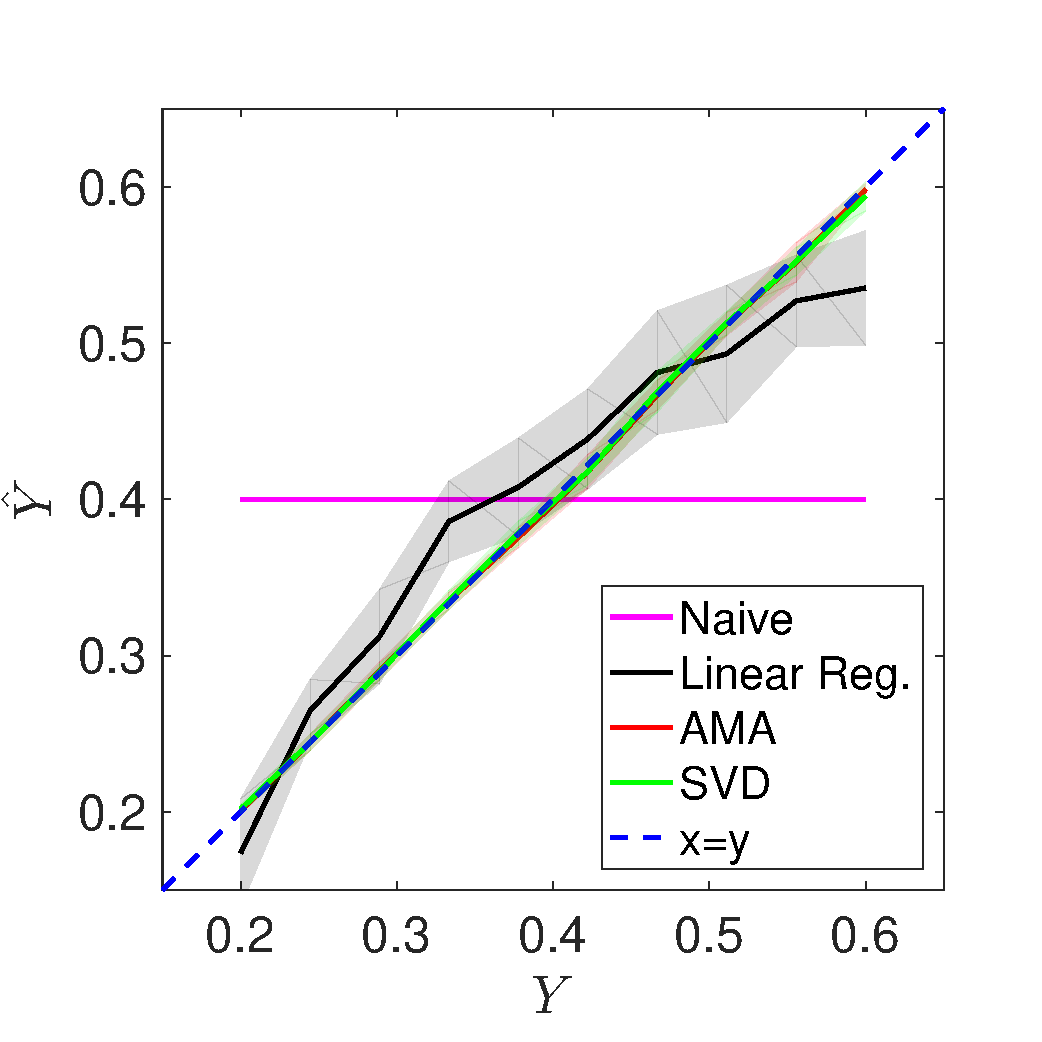
\includegraphics[width=\textwidth]{../Figures/Figure12/Figure12_d.pdf}
        \caption{Luminance Estimates}
        \label{fig:case10Results}
    \end{subfigure}
    \caption{{\bf Receptive fields and lightness estimates. Case 2:} Same as Fig. \ref{fig:case9AllResults}.}
    \label{fig:case10AllResults}
\end{figure}

% Figure 13
\begin{figure}
\centering
\begin{subfigure}[b]{0.27 \textwidth}
		\centering
        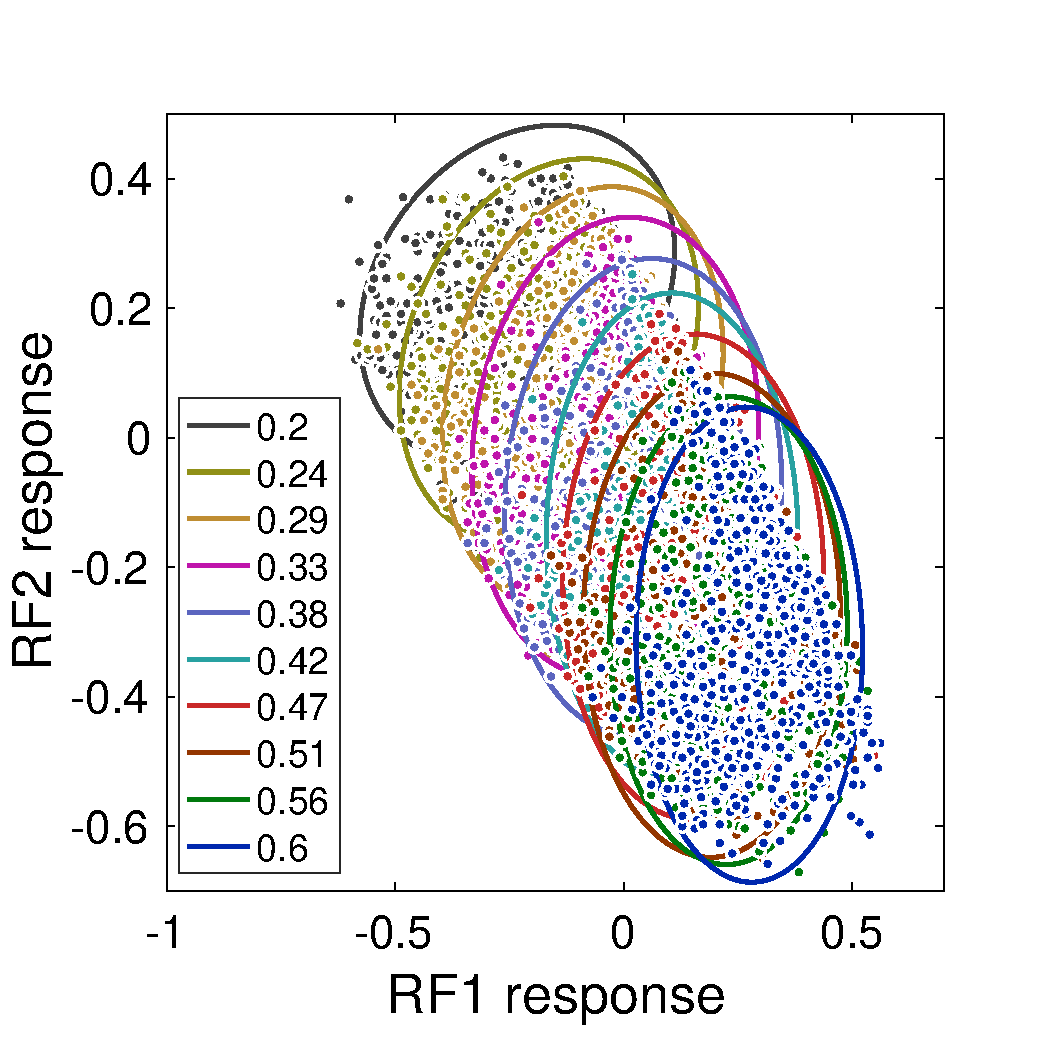
\includegraphics[width=\textwidth]{../Figures/Figure13/Figure13_a.pdf}
        \caption{SVD First 2 RFs}
        \label{fig:case12SVD}
    \end{subfigure}
    \begin{subfigure}[b]{0.27 \textwidth}   
        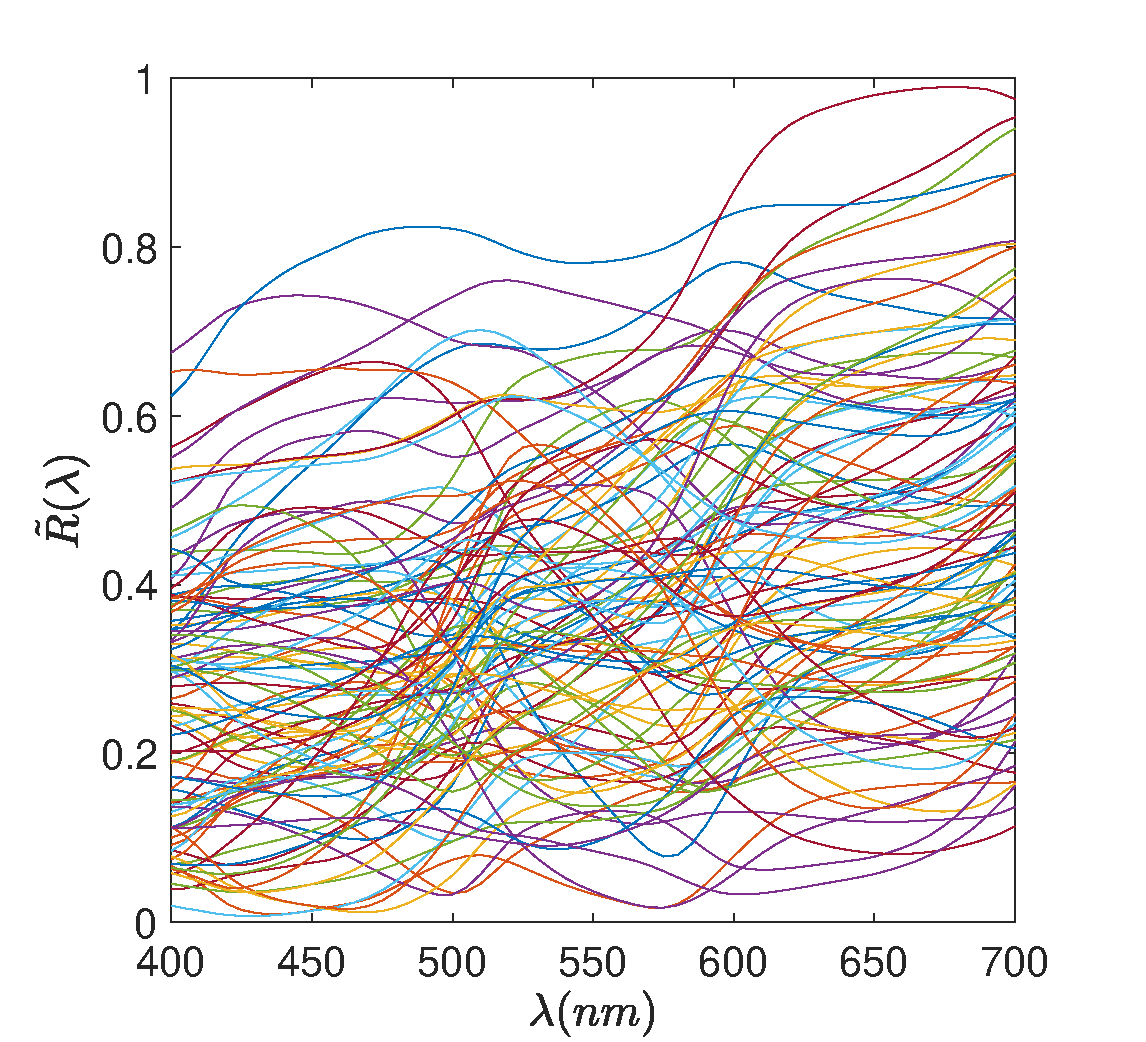
\includegraphics[width=\textwidth]{../Figures/Figure13/Figure13_b.pdf}
        \caption{AMA First 2 RFs}
        \label{fig:case12AMA}
    \end{subfigure}
        \begin{subfigure}[b]{0.20 \textwidth}
        
\includegraphics[width=\textwidth]{../Figures/Figure13/Figure13_c.pdf}
        \caption{AMA RF Response}
        \label{fig:case12FiltersResponse}
    \end{subfigure}    
        \begin{subfigure}[b]{0.2 \textwidth}
        \includegraphics[width=\textwidth]{../Figures/Figure13/Figure13_d.pdf}
        \caption{Luminance Estimates}
        \label{fig:case12Results}
    \end{subfigure}
    \caption{{\bf Receptive fields and lightness estimates. Case 3:}  Same as Fig. \ref{fig:case9AllResults}.}
    \label{fig:case12AllResults}
\end{figure}

\subsection{Lightness can be well estimated using a bayesian decoder with gaussian priors.}
We estimate the lightness of the target object in the images using the receptive field response of the corresponding contrast normalized cone responses. Fig.~ (\ref{fig:case9AllResults}-\ref{fig:case12AllResults})(c) shows the response of the first two RFs to the stimuli set for the three cases. For the training images at each lightness level, we approximate the receptive response of the contrast normalized cone responses by a multivariate gaussian. The target object lightness of an image in the test set is estimated using Bayesian decoder. We measure the estimation performance in terms of the relative root mean square ($E_{\rm rel}$) defined as:
\begin{align}
E_{\rm rel} = \sqrt{\left\langle\left(\frac{\hat{Y}-Y}{Y}\right)^2\right\rangle},
\end{align}
where $\hat{Y}$ corresponds to the estimated lightness and $Y$ to the assigned lightness. We use the first 8 RFs for lightness estimation ( see Fig.~\ref{fig:RMSEvsNFilters}).

Fig.~ (\ref{fig:case9AllResults}-\ref{fig:case12AllResults})(d) shows the lightness estimates and the RMSE for the three methods (Linear regression on center pixel, AMA and SVD). Additionally we show the estimate of a naive model that reports the mean value of the lightness labels used in the dataset. The diagonal x=y line is shown for reference. The shaded regions show $E_{\rm rel}$ for each method.

(Fig.~\ref{fig:summaryBarGraph}) compares the $E_{\rm rel}$ for the different methods for the three cases. Both AMA and SVD methods, which use the information from the entire image estimate the lightness better compared to linear regression which only uses the information from the center pixel. This shows the importance of context information for lightness estimation.

\subsection{The RFs of complex case generalize on simpler cases}
% Figure 8
\begin{figure}
\centering
\begin{subfigure}{0.3 \textwidth}
	\includegraphics[width=\textwidth]{../Figures/Figure14/Figure14_a.pdf}
	\caption{Performance of methods}
	\label{fig:summaryBarGraph}
    \end{subfigure}
    ~ %add desired spacing between images, e. g. ~, \quad, \qquad, \hfill etc. 
      %(or a blank line to force the subfigure onto a new line)
    \begin{subfigure}{0.3 \textwidth}   
	\includegraphics[width=\textwidth]{../Figures/Figure14/Figure14_b.pdf}
	\caption{SVD RF Performance}
	\label{fig:SVDBAR}
    \end{subfigure}
    ~ %add desired spacing between images, e. g. ~, \quad, \qquad, \hfill etc. 
    %(or a blank line to force the subfigure onto a new line)
        \begin{subfigure}{0.3 \textwidth}
	\includegraphics[width=\textwidth]{../Figures/Figure14/Figure14_c.pdf}
	\caption{AMA RF Performance}
	\label{fig:AMABAR}
    \end{subfigure}
\caption{{\bf Model and Filter Performance:} (a) Comparison of various methods on lightness estimations for the three cases studied here. For simple spectral variations, like where only the target reflectance varies (case 1) or only the target and illumination spectrum varies (Case 2), the lightness can be estimated well. This is so, because the lightness information can be estimated simply from the light reflected of the target( case 1) or from the contrast between the target and the {\it fixed} background (case 2). For more complex case, where the lightness information is confounded due to variations in target, background and illuminant (case 3), the estimation has higher variability. (b) Performance of the SVD receptive fields obtained from one case on the stimuli of others. The RFs obtained from any one of the three cases perform well on the stimuli from case 1. The RF of the most complicated case (case 3), has good performance on the stimuli of lower complexity. (c) Same as Fig.\ref{fig:SVDBAR} for AMA RFs.}
 \label{fig:barGraphs}
\end{figure}
Fig.~\ref{fig:SVDBAR} and Fig~\ref{fig:AMABAR} show the performance of the receptive fields learnt using the stimuli of one case on the stimuli of other cases. The RFs of case 3, (the most complex case) perform well on stimuli of case 1 and case 2.  Similarly, the RFs of case 2 performs well on the stimuli of case 1. Thus, the receptive fields leant on the complex case generalize for lightness estimation of stimuli for simpler cases.

\section{Discussion} \label{Discussion}
\section{Supplementary Information}


\subsection{Cone response to multispectral images}
Cone response to the multispectral images are generated
using \href{https://github.com/isetbio}{Isetbio}. The model incorporates several critical components of biological vision, including physiological optics, information about cornea, lens, pupil, etc. We simulate a model retinal mosaic with $51\times51$ cones having cone densities in the ratio [l,m,s]=[0.6 0.3 0.1]. The cone wavelength sensitivities are scaled such that the area under the sensitivity curve equals unity. A $51\times51$ pixel$^2$ patch of the image containing the target image is used to calculate the cone responses. The image patch is assumed to cover a $1^{\circ}$ field of view at a distance of 1 m.

\bibliography{references}
\bibliographystyle{jovcite}

\end{document}

